\section{Fase 7: Evaluación e Interpretación}
En esta fase, el \textit{Data Analysis Team} evalúa el modelo para comprender su calidad y garantizar que este aborda las preguntas generadas en el \textit{BCQM} de manera adecuada y completa. Es necesario que para realizar la evaluación se utilicen medidas especializadas basadas en el rendimiento, sensibilidad y especificidad del modelo. Adicionalmente, los resultados obtenidos deben ser entendibles por el medico experto en oncología, en donde se garantice que dichos resultados sean interpretados correctamente y estén relacionados a la estadificación y los biomarcadores del cáncer de mama. Es importante que el medico junto al científico de datos ajusten el modelo según las necesidades. Dado que se está trabajando con datos médicos sensibles, es necesario que al modelo final se aplique a un conjunto de validación para realizar una evaluación final. Además, el \textit{Data Analysis Team} puede asignar al modelo pruebas de \textit{significancia estadística} como prueba adicional para comprobar la respuesta obtenida a la pregunta generada. Esta prueba adicional es fundamental para justificar la implementación del modelo. Finalmente, dado que en el \textit{BCQM} se pueden plantear múltiples preguntas relacionadas a diferentes tipos de cáncer de mama y técnicas de diagnóstico durante el \textit{Release}, es necesario que los científicos con ayuda del ingeniero de datos unan, si es posible, los resultados obtenidos en una matriz o mapa de calor para identificar el coeficiente de correlación entre dos o más variables oncológicas. Esta matriz resultante debe ser analizada por el medico experto en oncología para determinar si existe una relación significativa entre los diferentes tipos de cáncer de mama.

Con base a los resultados obtenidos en la fase anterior, el modelo \textit{BIRCH} fue el seleccionado para agrupar los datos genómicos del conjunto de datos del carcinoma invasivo de mama (TCGA, Cell 2015) en \textit{clusters} basados en los tipos de cáncer lobulillar invasivo(ILC), ductal invasivo(IDC) o de tumores mixtos(MDLC).

\subsection{Agrupamiento BIRCH}
El método de agrupación de datos \textit{BIRCH}(Balanced, Iterative Reducing , and Clustering using Hierarchies) reúne de forma incremental y dinámica puntos de datos métricos multidimensionales entrantes para intentar producir una agrupación de mejor calidad con los recursos disponibles, es decir, la memoria disponible y las limitaciones de tiempo. Por lo general, BIRCH puede encontrar una buena agrupación con una sola exploración de los datos y mejorar aún más la calidad con unas pocas exploraciones adicionales. BIRCH es también el primer algoritmo de clustering propuesto en el área de bases de datos que maneja eficazmente el \textit{“ruido”}, es decir puntos de datos que no forman parte del patrón subyacente \cite{Zhang1996}. 

Este modelo, presentó un mayor desempeño al medir la eficiencia espacio-temporal, la sensibilidad al orden de entrada de los datos y la calidad de la agrupación mediante varias iteraciones. El resultado obtenido puede ser observado en la figura \ref{BIRCH_TSNE} generada con el método T-SNE que permite visualizar las similitudes entre vecinos en un espacio multidimensional y la figura \ref{BIRCH_PCA} que permite visualizar la distancia entre clusters según el análisis de componentes principales (PCA\footnote{PCA: Principal Component Analysis}). Dado lo anterior, en las gráficas se visualizo que los clusters presentaban una métrica de cohesión y separación que permitió identificar las 4 agrupaciones generadas por el modelo BIRCH.

\begin{figure}
	\centering
	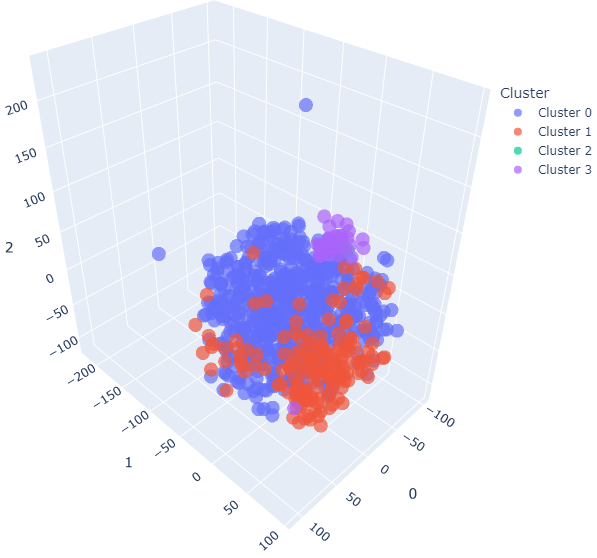
\includegraphics[width=0.5
	\linewidth]{NOTEBOOK/IMAGENES_CLUSTERING/8_TNSE_Birch_Clustering}
	\caption{T-SNE generado por el modelo BIRCH.}
	\label{BIRCH_TSNE}
\end{figure}

\begin{figure}
	\centering
	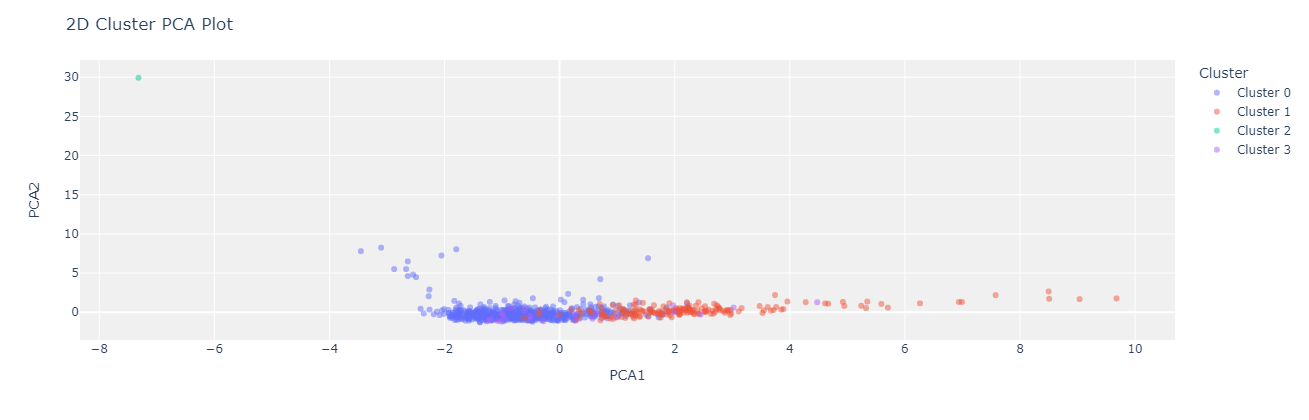
\includegraphics[width=1
	\linewidth]{NOTEBOOK/IMAGENES_CLUSTERING/8_PCA_Birch_Clustering}
	\caption{PCA generado por el modelo BIRCH.}
	\label{BIRCH_PCA}
\end{figure}

\subsection{Métricas para la validación del Clustering}
Como se afirmo anteriormente, en esta fase se realizó la evaluación de los resultados obtenidos por el modelo \textit{BIRCH}. Conviene subrayar, que la validación externa y la validación interna son las dos categorías más importantes para la validación de los modelos de agrupamiento. La principal diferencia es si se usa o no información externa para la validación, es decir, información que no es producto de la técnica de agrupación utilizada\cite{Elizabeth2023}. Dada la naturaleza del algoritmo y de lo datos, en este caso se utilizó \textit{validación interna} para medir el clustering generado por el modelo BIRCH únicamente basados en información de los datos del carcinoma invasivo de mama (TCGA, Cell 2015), lo cual nos permitió evaluar que tan buena fue la estructura del clustering sin necesidad de información ajena al propio algoritmo y su resultado. Como el objetivo del clustering es agrupar objetos similares en el mismo clúster y objetos diferentes ubicarlos en diferentes clusters, las métricas de validación interna están basadas usualmente en los dos siguientes criterios\cite{Elizabeth2023}:
\begin{itemize}[label=\HandRight]
	\item \textbf{Cohesión}: El miembro de cada clúster debe ser lo más cercano posible a los otros miembros del mismo clúster.
	\item \textbf{Separación}: Los clusters deben estar ampliamente separados entre ellos.
\end{itemize}
Dado lo anterior, se seleccionaron las siguientes métricas de validación internas:
%-------------------------------------------
\subsubsection{Indice de Davies-Bouldien}
Este índice representa el promedio de las distancias que pertenecen a un determinado cluster.	Valores pequeños para el índice $DB$ indica clústeres compactos, y cuyos centros están bien separados los unos de los otros. Consecuentemente el número de clústeres que minimiza el índice Davies-Bouldien se toma como el óptimo. Dado lo anterior, este índice está definido como:
\begin{equation}
	DB = \frac{1}{k} \sum_{i=1,i\neq j}^{k} max \left( \frac{\sigma_{i}+\sigma_{j}}{d(c_{i},c_{j})}\right) 
\end{equation}
\begin{itemize}[label=]
	\item $k=$ número de clústeres.
	\item $\sigma_{i}=$ distancia promedio entre cada punto en el clúster $i$ y el centroide del clúster.
	\item $\sigma_{j}=$ distancia promedio entre cada punto en el clúster $j$ y el centroide del clúster.
	\item $d(c_{i},c_{j})=$ distancia entre los centroides de los 2 clústeres .
\end{itemize}
%-------------------------------------------
\subsubsection{Coeficiente de silhouette} 
Esta métrica permite identificar cual es el número óptimo de agrupamientos. Dado lo anterior, está definido como:
\begin{itemize}[label=]
	\item $a(x)=$ distancia promedio de $x$ a todos los demás puntos en el mismo cluster.
	\item $b(x)=$ distancia promedio de $x$ a todos los demás puntos en el cluster más cercano.
\end{itemize}
Dado esto, se dice que el coeficiente de la silueta para $x$ está dado por:
\begin{equation}
	s(x) = \frac{b(x)-a(x)}{max\left\lbrace a(x), b(x) \right\rbrace }
\end{equation}

Donde el valor de $s(x)$ puede variar entre $-1$ y $1$. En donde, $-1$ es interpretado como un mal agrupamiento, $0$ como un resultado indiferente y $1$ como un buen agrupamiento \cite{Ramirez2018}. Por lo tanto, el coeficiente de la silueta para todo el agrupamiento es:

\begin{equation}
	SC = \frac{1}{N} \sum_{i = 1}^{N}s(x)
\end{equation}
%-------------------------------------------
\subsubsection{Método del codo}
Esta métrica utiliza los valores de la inercia obtenidos tras aplicar el algoritmo de agrupamiento a diferente número de clusters (desde $1$ a $N$ clusters), siendo la inercia la suma de las distancias al cuadrado de cada objeto del cluster a su centroide:

\begin{equation}
	inercia = \sum_{i = 0}^{N}  \parallel x_{i} - \mu  \parallel
\end{equation}

Una vez obtenidos los valores, se representa en una gráfica lineal la inercia respecto del número de clusters. En esta gráfica se debería apreciar un cambio brusco en la evolución de la inercia, teniendo la línea representada una forma similar a la de un brazo y su codo. El punto en el que se observa ese cambio nos indica el número óptimo de clusters a seleccionar para el conjunto de datos en cuestión \cite{Moya2022}. 

%-------------------------------------------
\subsection{Evaluación del modelo BIRCH}
Con base a las métricas de validación internas aplicadas al modelo BIRCH, se obtuvo un índice de Davies-Bouldien del $1.8703$, valor que ratifico que lo centros estaban separados correctamente, tal y como se observa en la tabla \ref{Davies-Bouldien}. Adicionalmente, en la figura \ref{a} se observa los 4 clusters generados por el modelo para un coeficiente de Silhouette del $0.1286$. Por último, en la figura \ref{b} se observa que la inercia se produce en $k = 5 $, corroborando el resultado del coeficiente de Silhouette obtenido anteriormente y confirmando que el modelo tenia un número de clusters adecuado. Por consiguiente, se infirió que el modelo presentaba clústeres compactos con centros considerablemente separados los unos de los otros lo cual indico que el agrupamiento generado para el conjunto de datos del carcinoma invasivo de mama era aceptable. 

\begin{table*}[!htb]
	\footnotesize
	\centering
	\begin{threeparttable}
		\begin{tabular}{p{1cm} p{4cm} p{2.5cm} p{2.5cm} p{1.5cm}} \toprule	
			\begin{center}Id\end{center}
			&\begin{center}Modelo Clustering\end{center}
			&\begin{center}Silhouette\end{center}
			&\begin{center}Davies-Bouldin\end{center}
			&\begin{center}Clusters\end{center}
			\\ \hline 8 & BIRCH Clustering	&	0,1286	&	1,8703	&	4
			\\ \hline
		\end{tabular}
		\caption{Indice de Davies-Bouldien del modelo BIRCH.}
		\label{Davies-Bouldien}
	\end{threeparttable}
\end{table*}

\begin{figure}[!htb]
	\centering
	\subfloat[Coeficiente de Silhouette]{\label{a}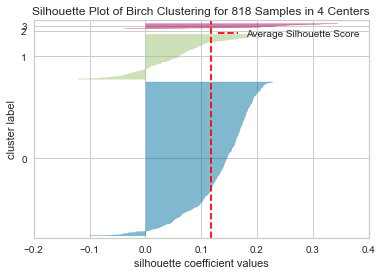
\includegraphics[width=0.5\linewidth]{NOTEBOOK/IMAGENES_CLUSTERING/8_SILHOUTETTE_Birch_Clustering}}\hfill
	\subfloat[Método del codo]{\label{b}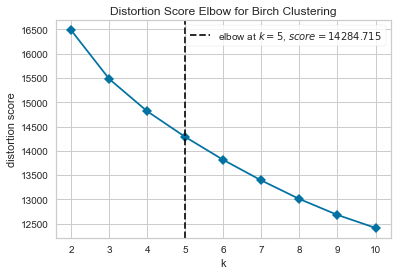
\includegraphics[width=0.5\linewidth]{NOTEBOOK/IMAGENES_CLUSTERING/8_ELBOW_Birch_Clustering}}\par 
	\caption{Métricas de validación internas modelo de agrupamiento BIRCH}
	\label{Silhouette_Elbow}
\end{figure}

\clearpage
%-------------------------------------------
\subsection{Interpretación de los resultados}
Con base a los 4 \textit{clusters} generados por el modelo \textit{BIRCH}, se procedió a identificar las características de origen genómico compartidas por 818 pacientes para analizar su comportamiento y así dar respuesta a las preguntas generadas en el BCQM. Dado lo anterior, se generó un análisis diagnostico para determinar las causas de las tendencias y las correlaciones de dichas variables con los tipos de cáncer de mama Lobulillar Invasivo (ILC), Ductal Invasivo (IDC) y Tumores Mixtos (MDLC). Se debe agregar que los clusters estaban conformados por 41 variables distribuidas en 9 variables numéricas y 33 variables categóricas, en donde el \textit{Cluster 0} agrupo 615 pacientes, el \textit{Cluster 1} agrupo 180 pacientes, el \textit{Cluster 2} agrupo 1 paciente y el \textit{Cluster 3} agrupo 22 pacientes. Los detalles de lo agrupación de los clusters por variable se pueden observar en la tabla \ref{clusters}:
\begin{table}[!htb]
	\begin{center} 
		\begin{tabular}{ |c|c|c|c| }
			\hline 
			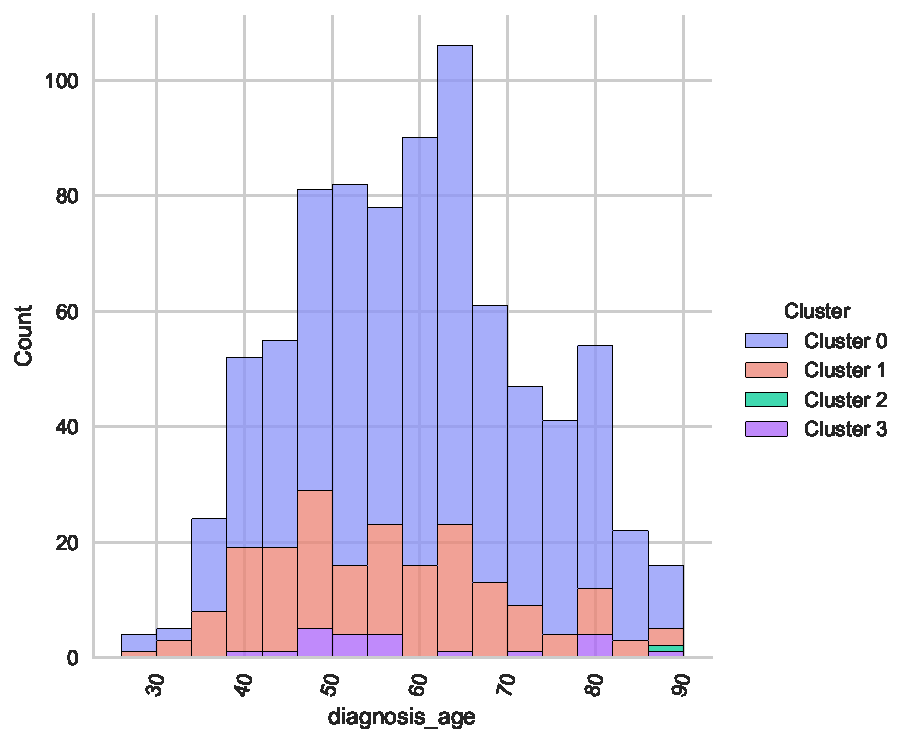
\includegraphics[width=0.21\textwidth]{NOTEBOOK/IMAGENES_BIRCH_DESCRIPTIVAS/1} 
			& 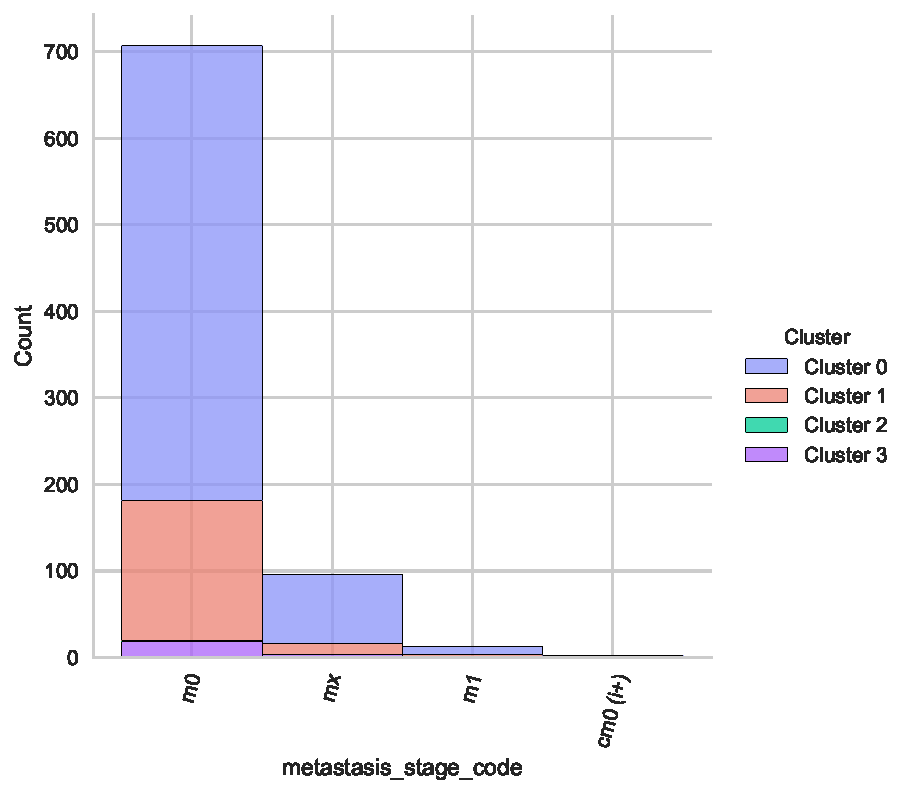
\includegraphics[width=0.21\textwidth]{NOTEBOOK/IMAGENES_BIRCH_DESCRIPTIVAS/2} 
			& 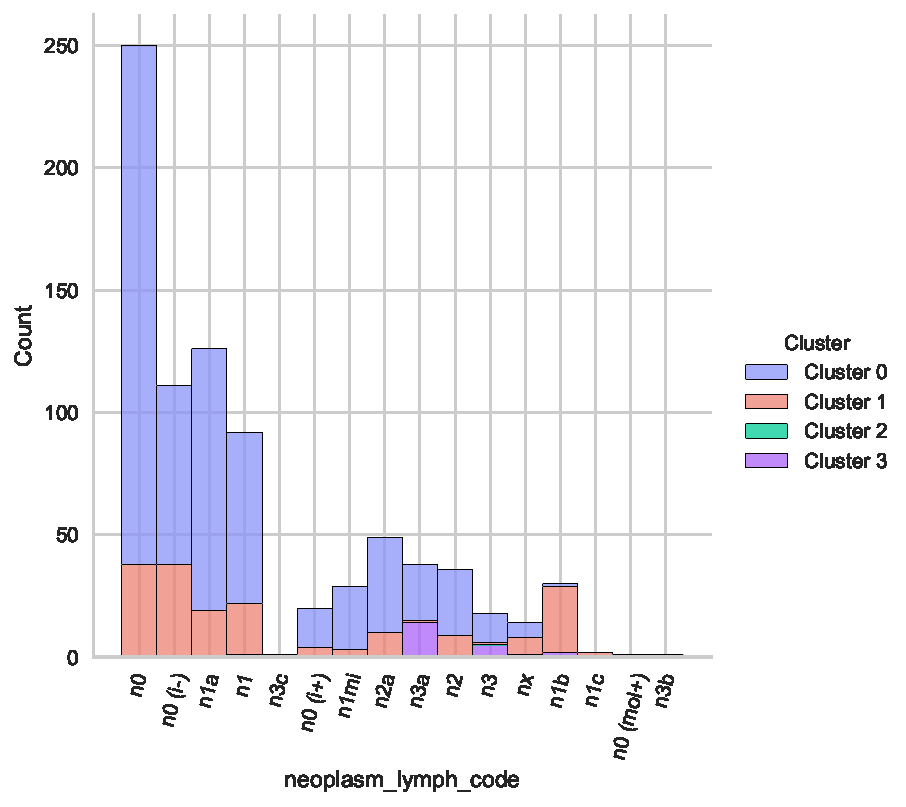
\includegraphics[width=0.21\textwidth]{NOTEBOOK/IMAGENES_BIRCH_DESCRIPTIVAS/3}
			& 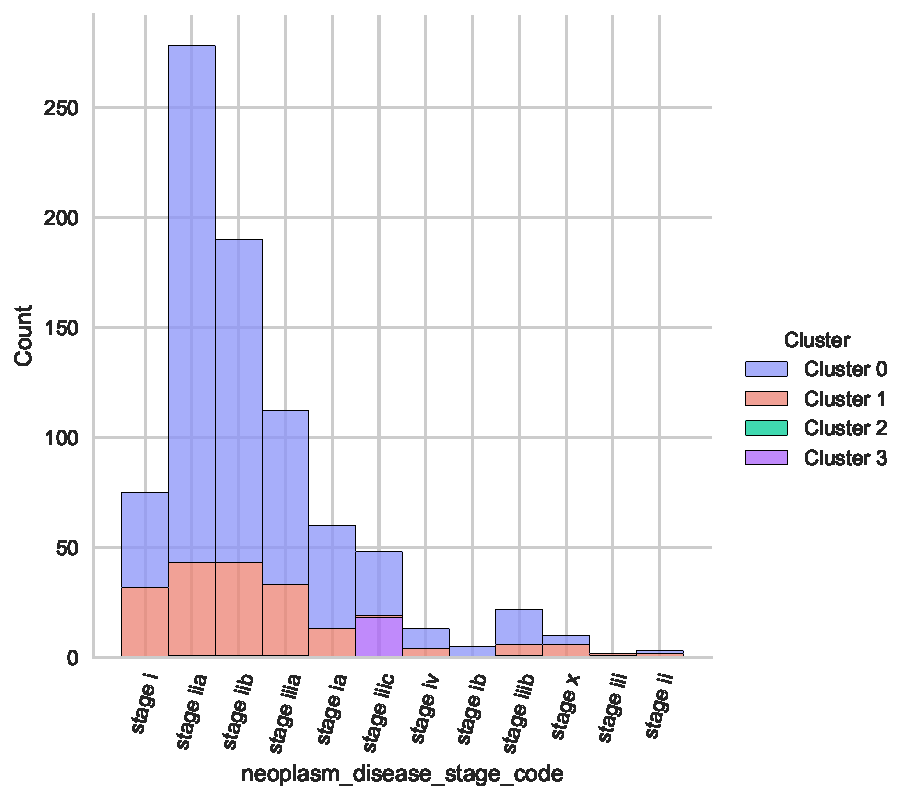
\includegraphics[width=0.21\textwidth]{NOTEBOOK/IMAGENES_BIRCH_DESCRIPTIVAS/4} 
			\\  \hline 
			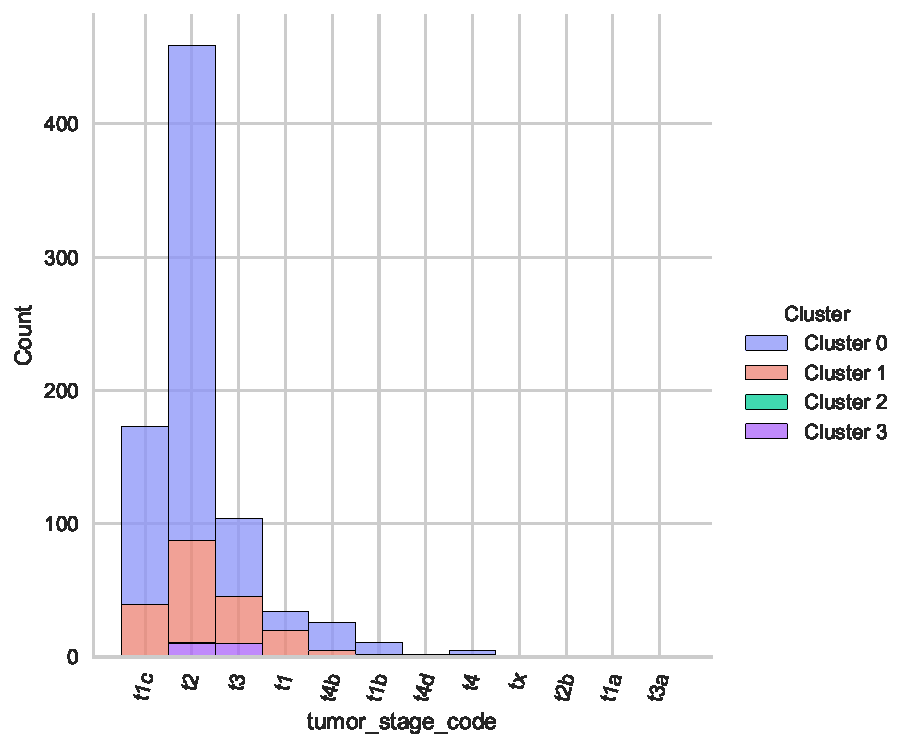
\includegraphics[width=0.21\textwidth]{NOTEBOOK/IMAGENES_BIRCH_DESCRIPTIVAS/5} 
			& 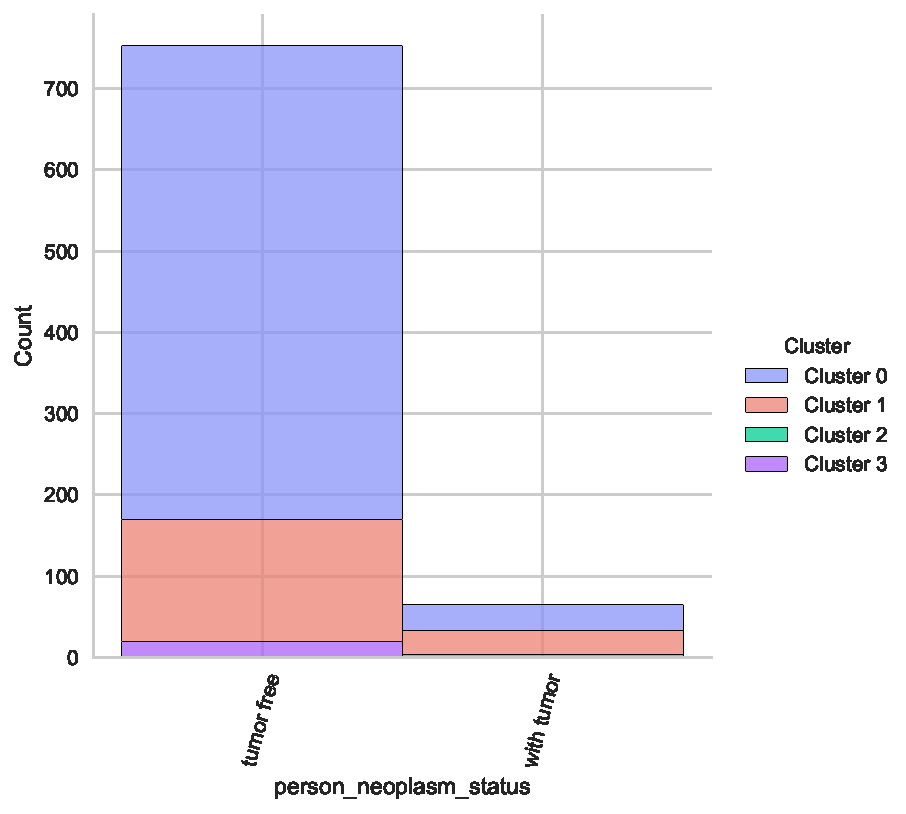
\includegraphics[width=0.21\textwidth]{NOTEBOOK/IMAGENES_BIRCH_DESCRIPTIVAS/41} 
			& 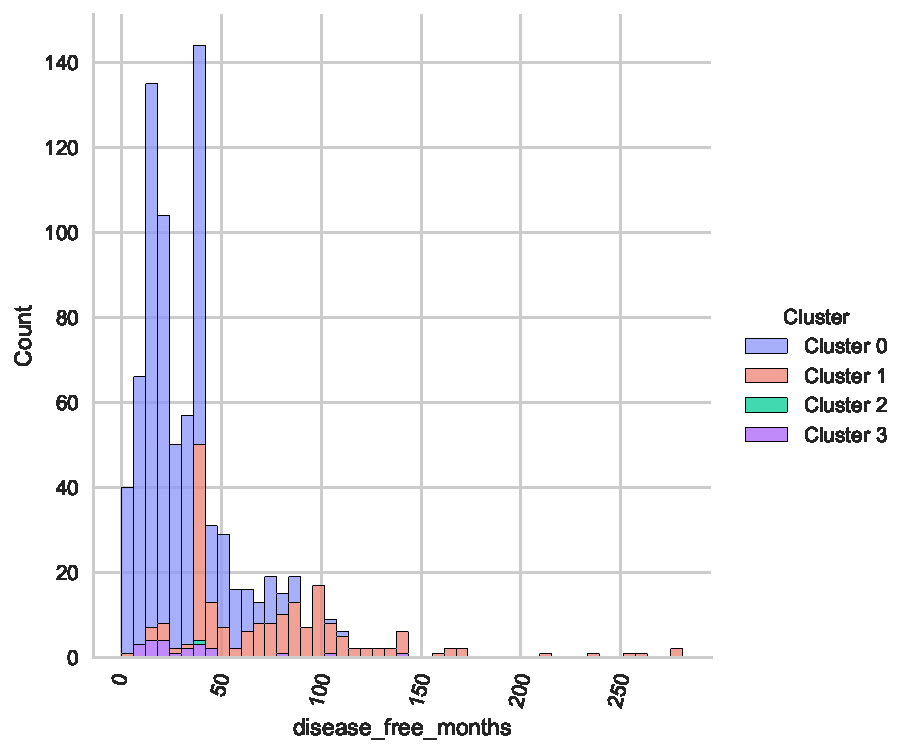
\includegraphics[width=0.21\textwidth]{NOTEBOOK/IMAGENES_BIRCH_DESCRIPTIVAS/7} 
			& 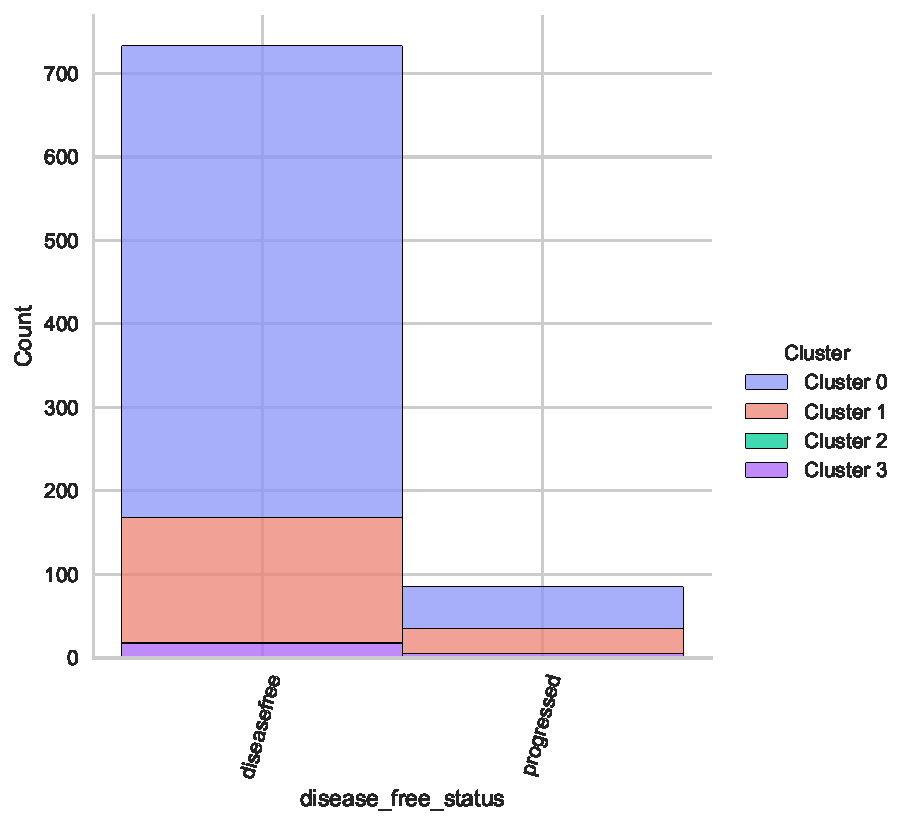
\includegraphics[width=0.21\textwidth]{NOTEBOOK/IMAGENES_BIRCH_DESCRIPTIVAS/8} 
			\\  \hline 
			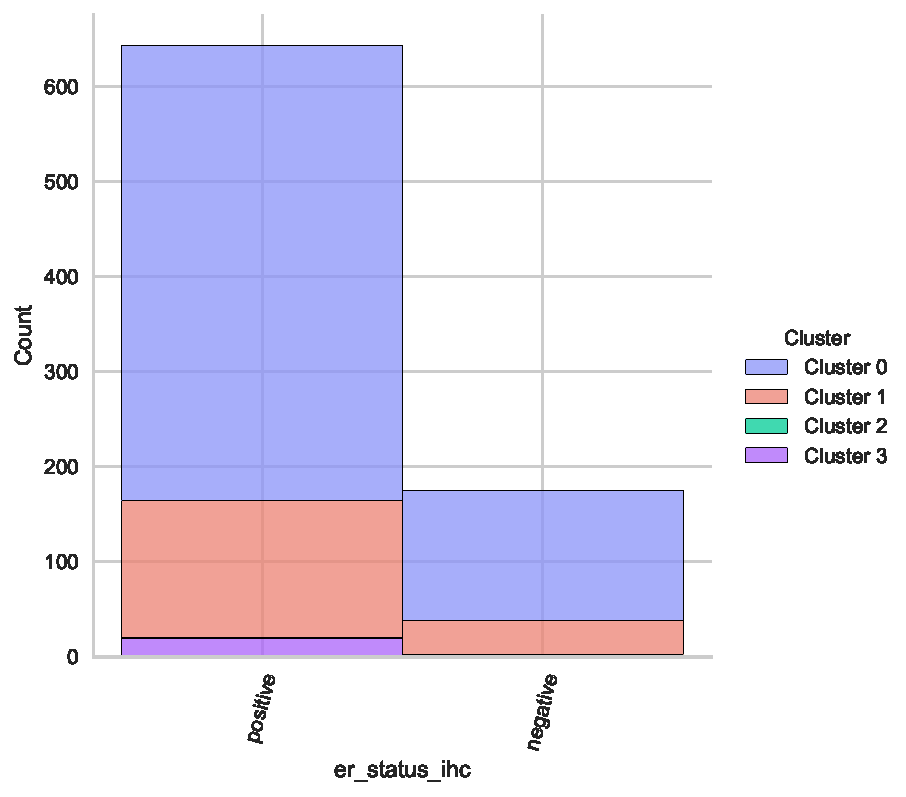
\includegraphics[width=0.21\textwidth]{NOTEBOOK/IMAGENES_BIRCH_DESCRIPTIVAS/9} 
			& 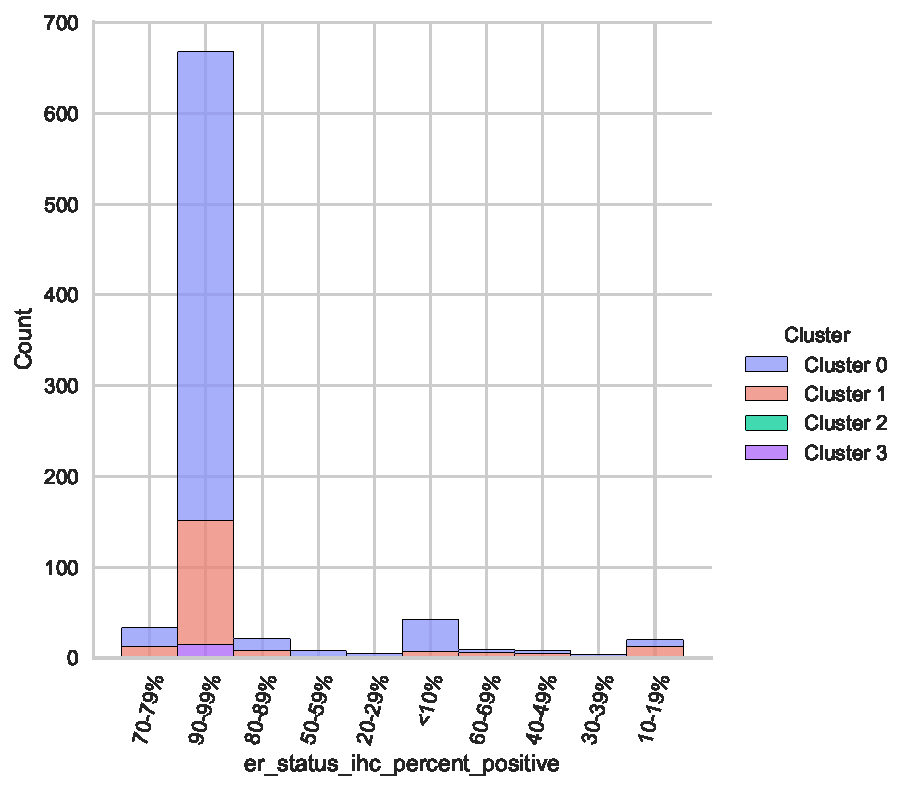
\includegraphics[width=0.21\textwidth]{NOTEBOOK/IMAGENES_BIRCH_DESCRIPTIVAS/10} 
			& 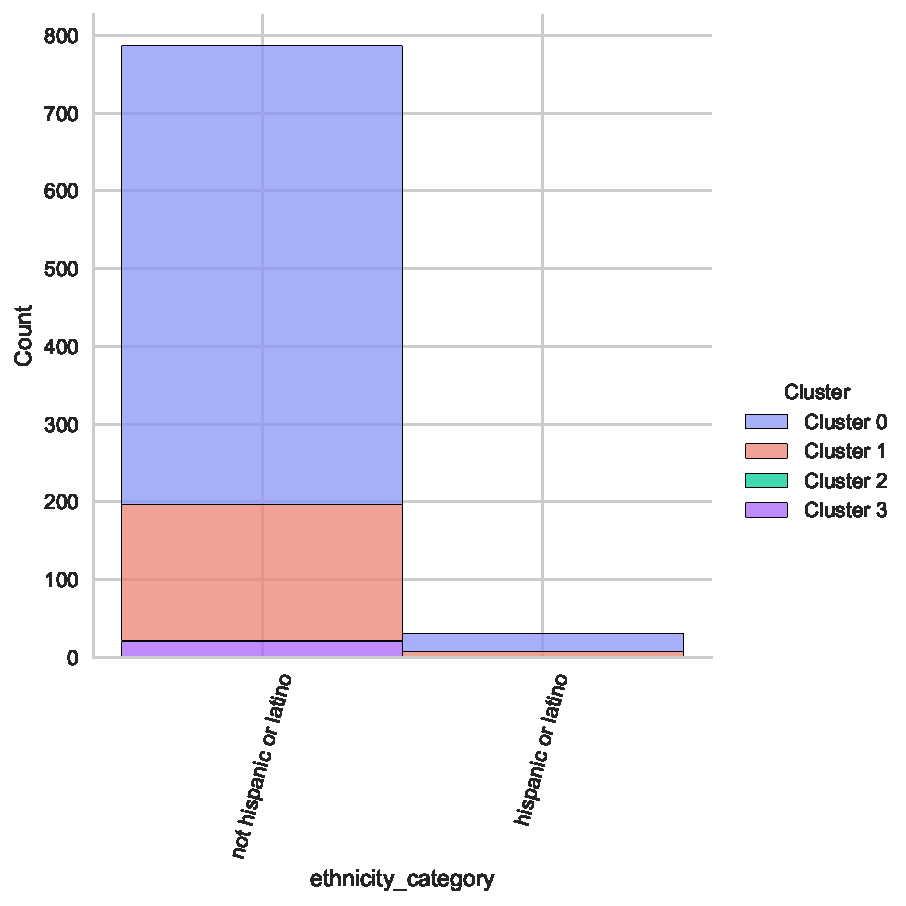
\includegraphics[width=0.21\textwidth]{NOTEBOOK/IMAGENES_BIRCH_DESCRIPTIVAS/11} 
			& 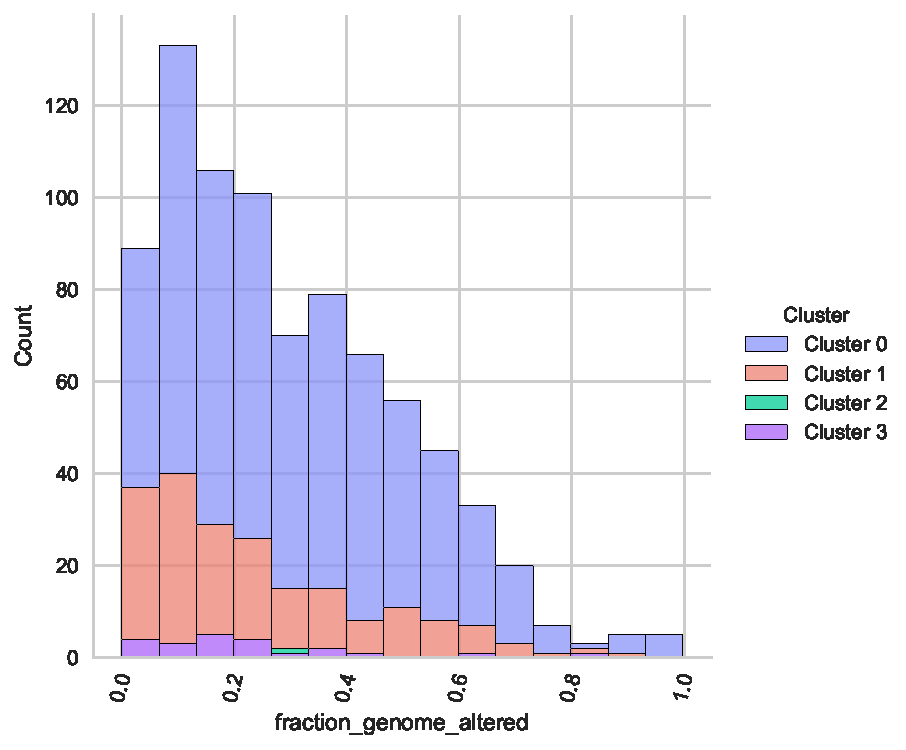
\includegraphics[width=0.21\textwidth]{NOTEBOOK/IMAGENES_BIRCH_DESCRIPTIVAS/12} 
			\\  \hline 
			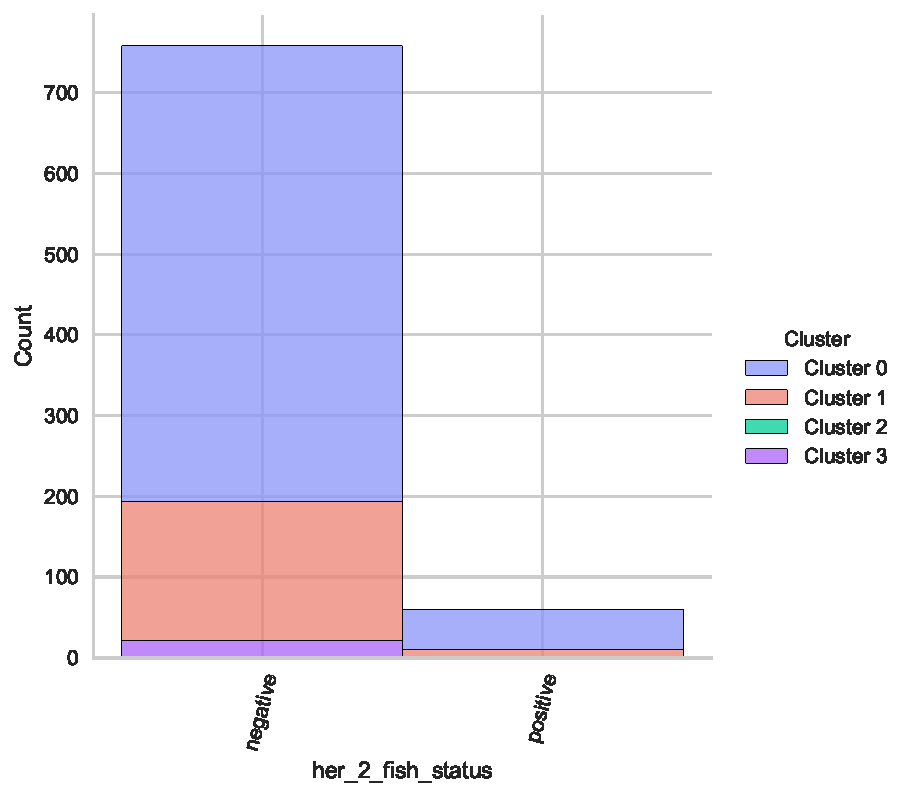
\includegraphics[width=0.21\textwidth]{NOTEBOOK/IMAGENES_BIRCH_DESCRIPTIVAS/13} 
			& 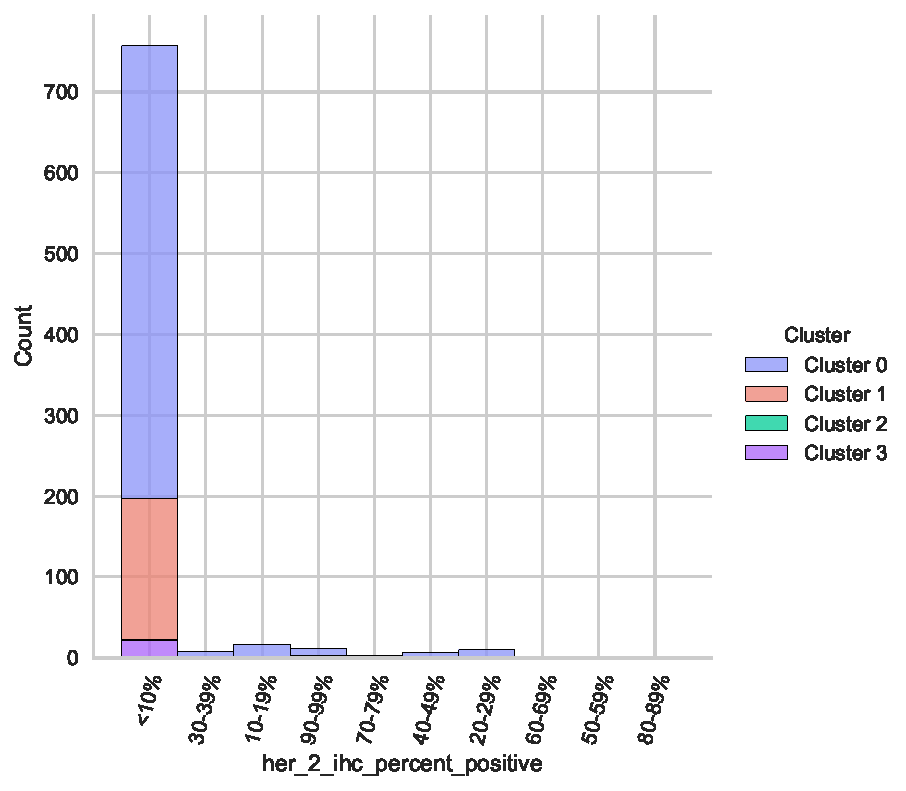
\includegraphics[width=0.21\textwidth]{NOTEBOOK/IMAGENES_BIRCH_DESCRIPTIVAS/14} 
			& 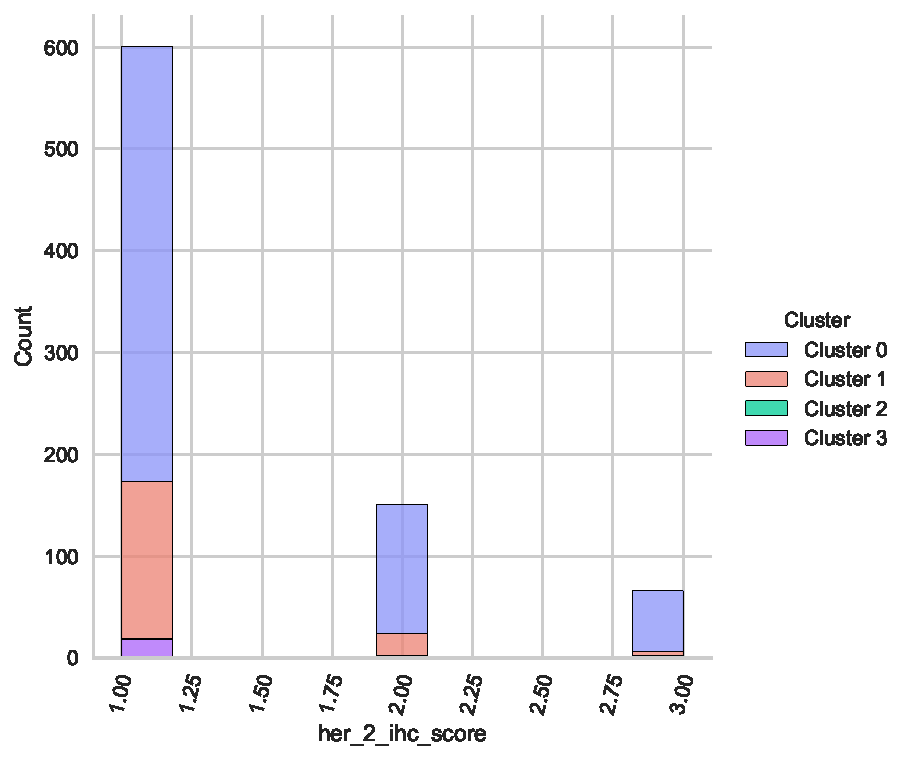
\includegraphics[width=0.21\textwidth]{NOTEBOOK/IMAGENES_BIRCH_DESCRIPTIVAS/15} 
			& 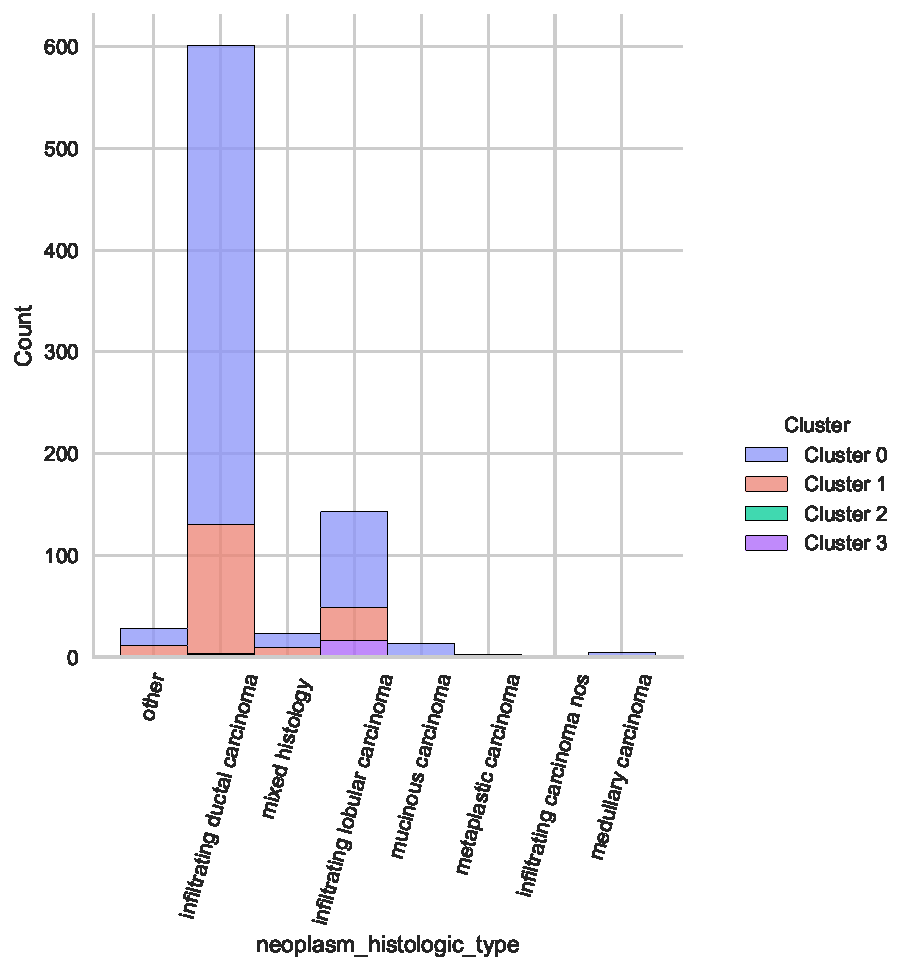
\includegraphics[width=0.21\textwidth]{NOTEBOOK/IMAGENES_BIRCH_DESCRIPTIVAS/16} 
			\\  \hline    
		\end{tabular} 
	\end{center} 
\end{table}

\begin{table}
	\begin{center} 
		\begin{tabular}{ |c|c|c|c| }
			\hline 
			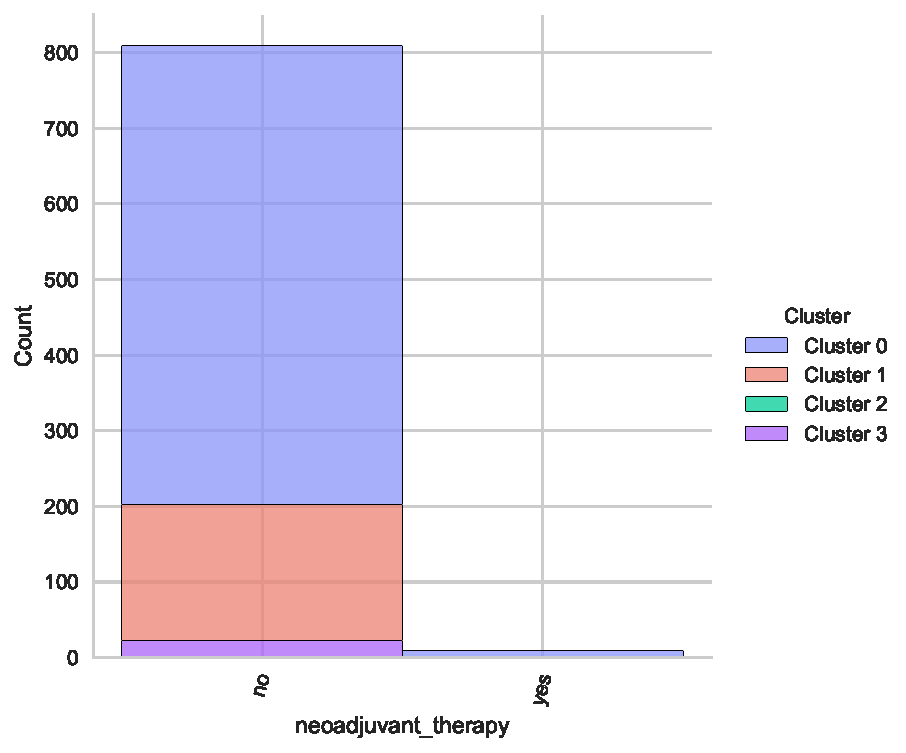
\includegraphics[width=0.22\textwidth]{NOTEBOOK/IMAGENES_BIRCH_DESCRIPTIVAS/17} 
			& 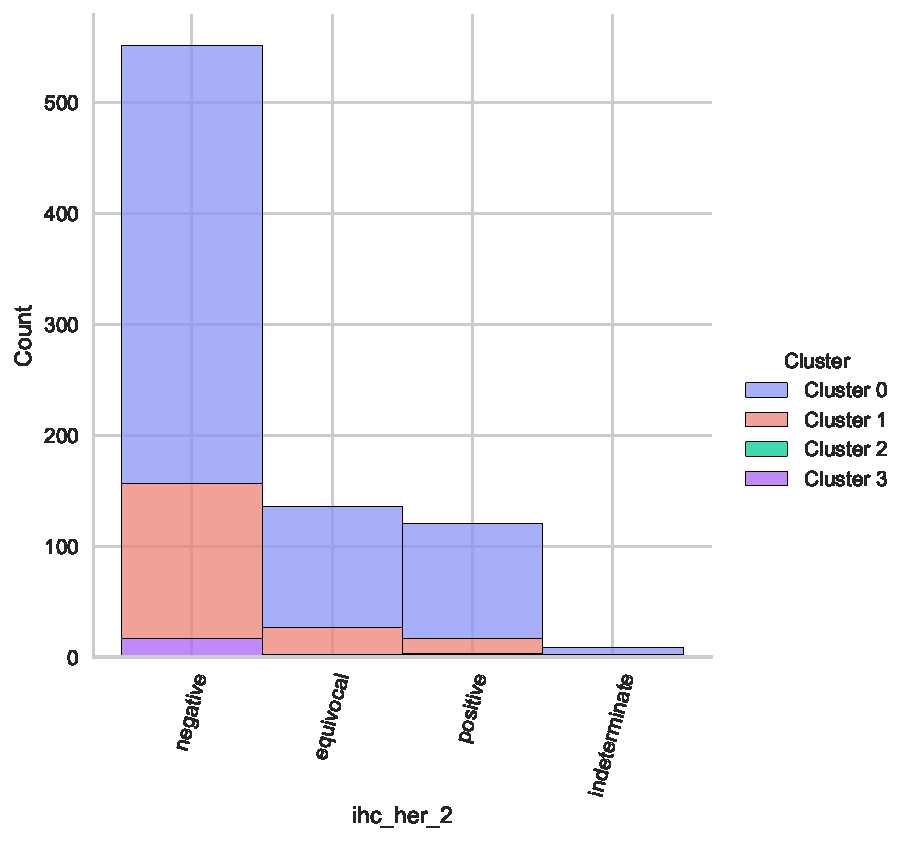
\includegraphics[width=0.22\textwidth]{NOTEBOOK/IMAGENES_BIRCH_DESCRIPTIVAS/18} 
			& 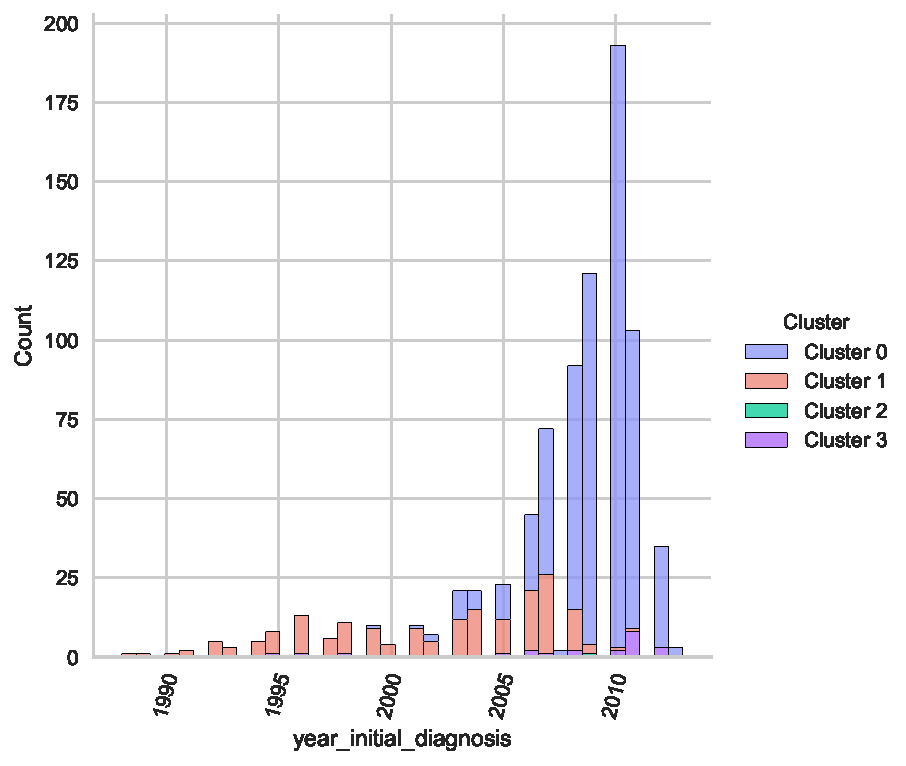
\includegraphics[width=0.22\textwidth]{NOTEBOOK/IMAGENES_BIRCH_DESCRIPTIVAS/19} 
			& 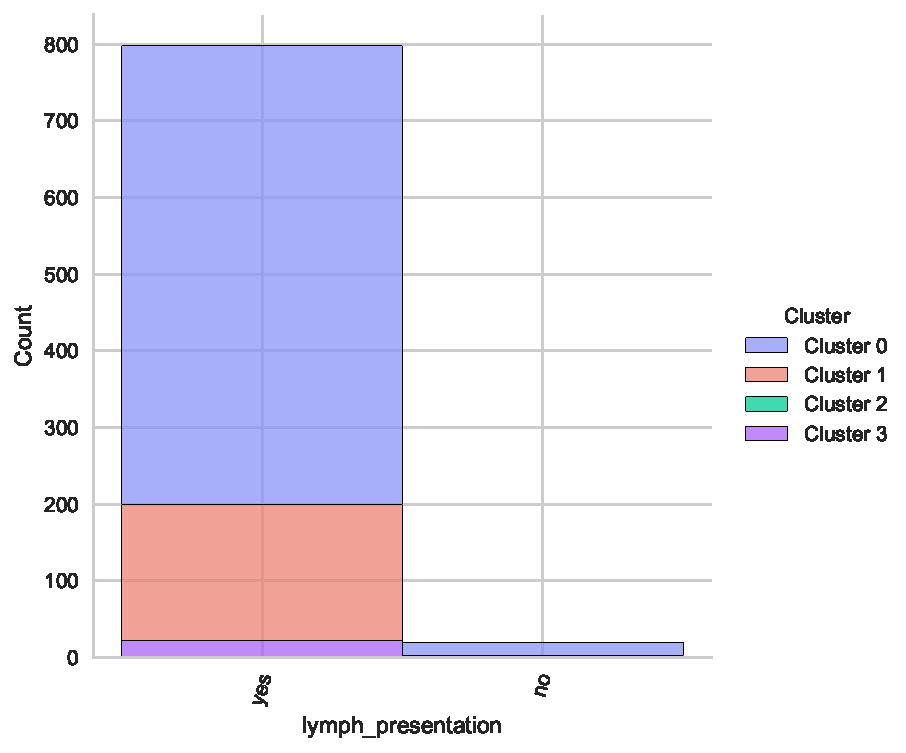
\includegraphics[width=0.22\textwidth]{NOTEBOOK/IMAGENES_BIRCH_DESCRIPTIVAS/20} 
			\\  \hline
			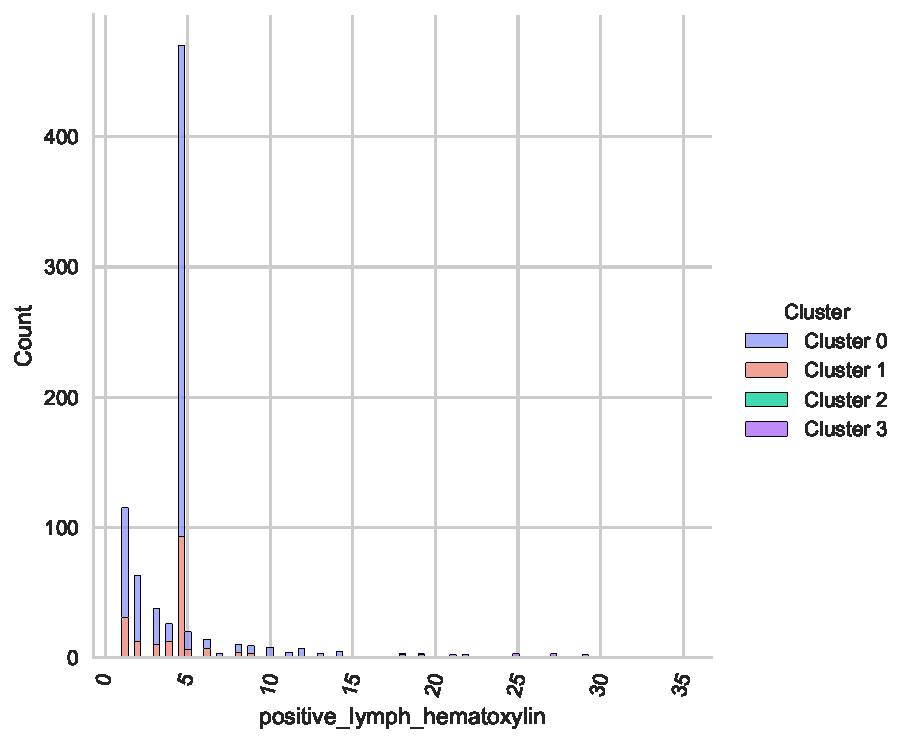
\includegraphics[width=0.22\textwidth]{NOTEBOOK/IMAGENES_BIRCH_DESCRIPTIVAS/21} 
			& 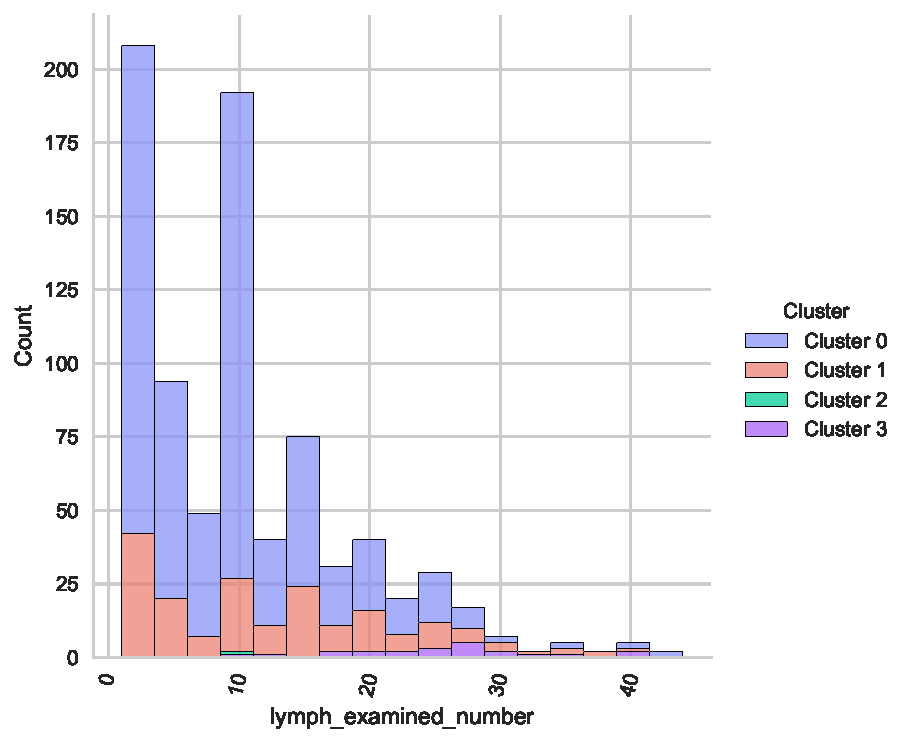
\includegraphics[width=0.22\textwidth]{NOTEBOOK/IMAGENES_BIRCH_DESCRIPTIVAS/22} 
			& 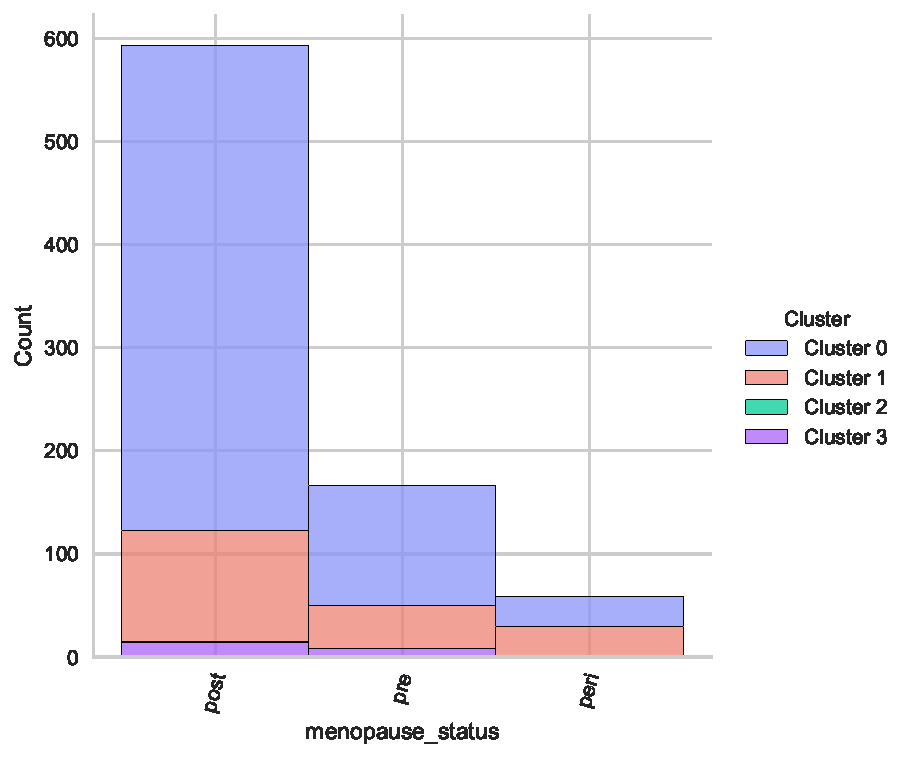
\includegraphics[width=0.22\textwidth]{NOTEBOOK/IMAGENES_BIRCH_DESCRIPTIVAS/23} 
			& 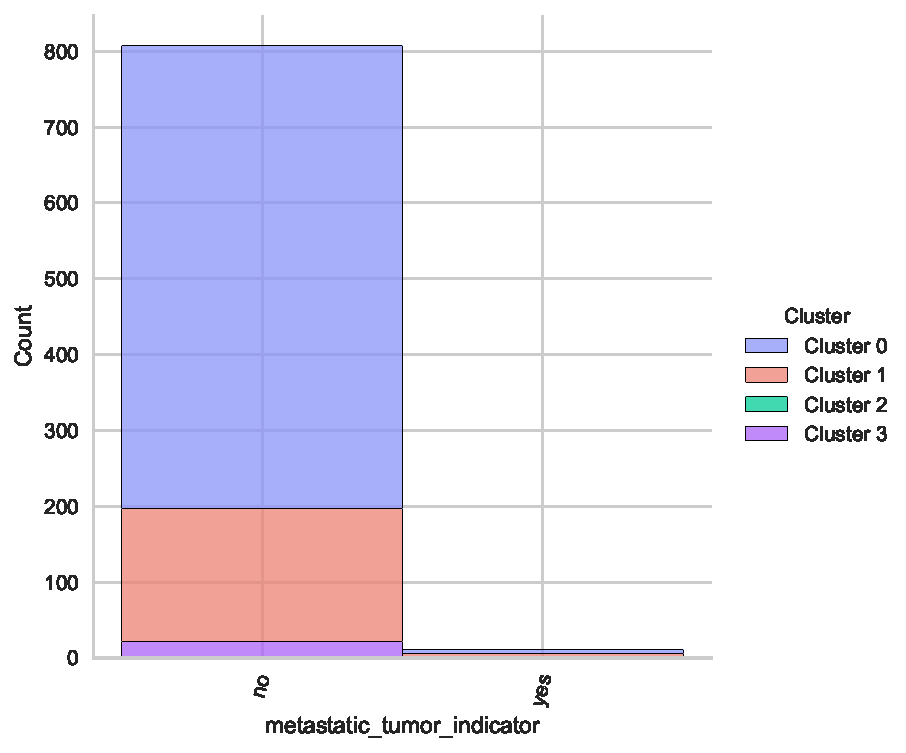
\includegraphics[width=0.22\textwidth]{NOTEBOOK/IMAGENES_BIRCH_DESCRIPTIVAS/24} 
			\\  \hline 
			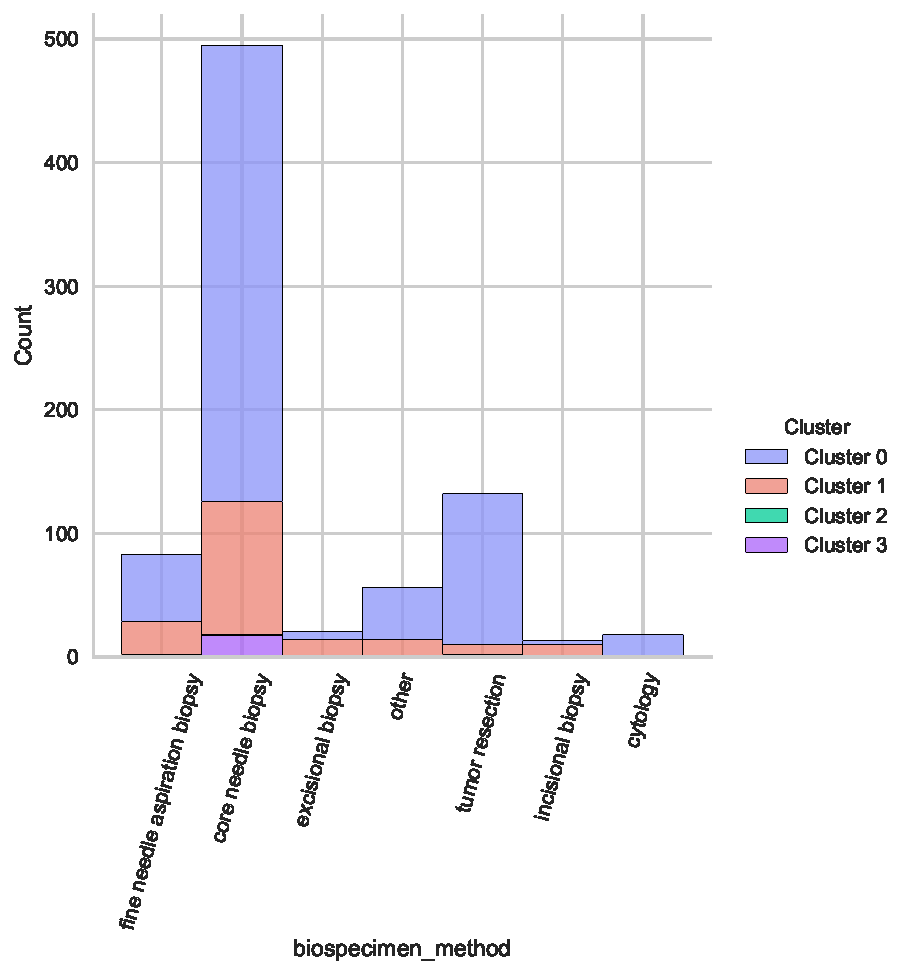
\includegraphics[width=0.22\textwidth]{NOTEBOOK/IMAGENES_BIRCH_DESCRIPTIVAS/25} 
			& 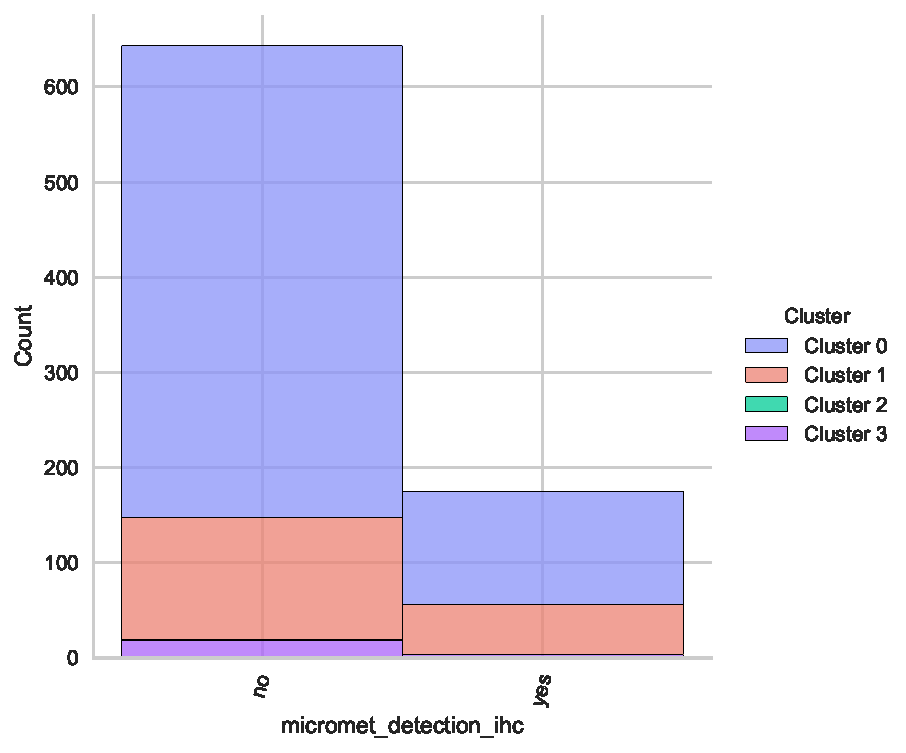
\includegraphics[width=0.22\textwidth]{NOTEBOOK/IMAGENES_BIRCH_DESCRIPTIVAS/26} 
			& 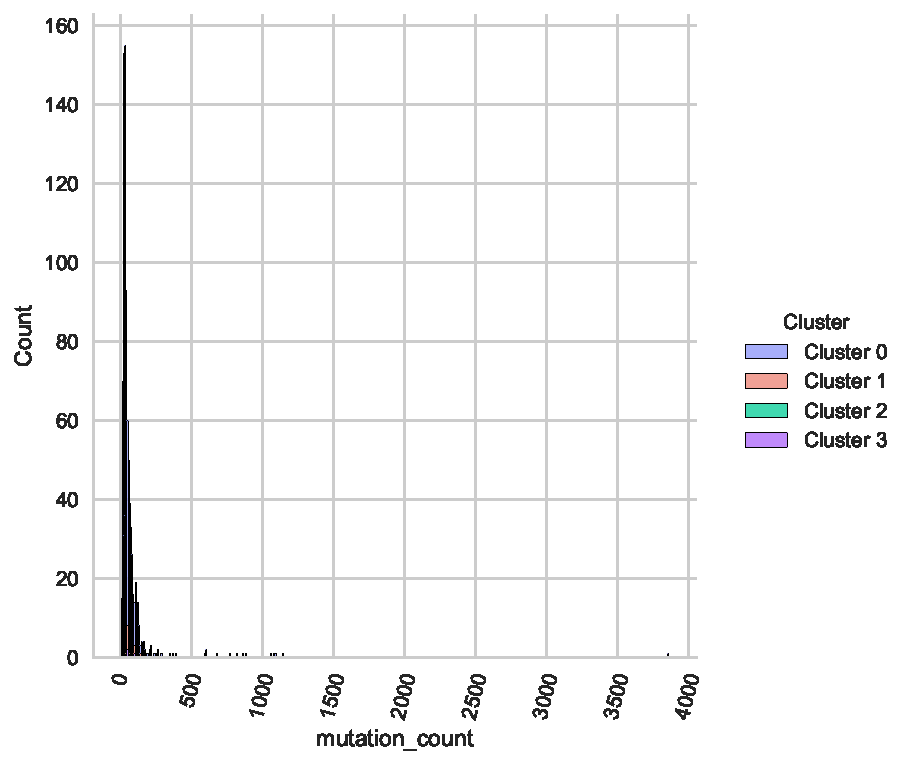
\includegraphics[width=0.22\textwidth]{NOTEBOOK/IMAGENES_BIRCH_DESCRIPTIVAS/27} 
			& 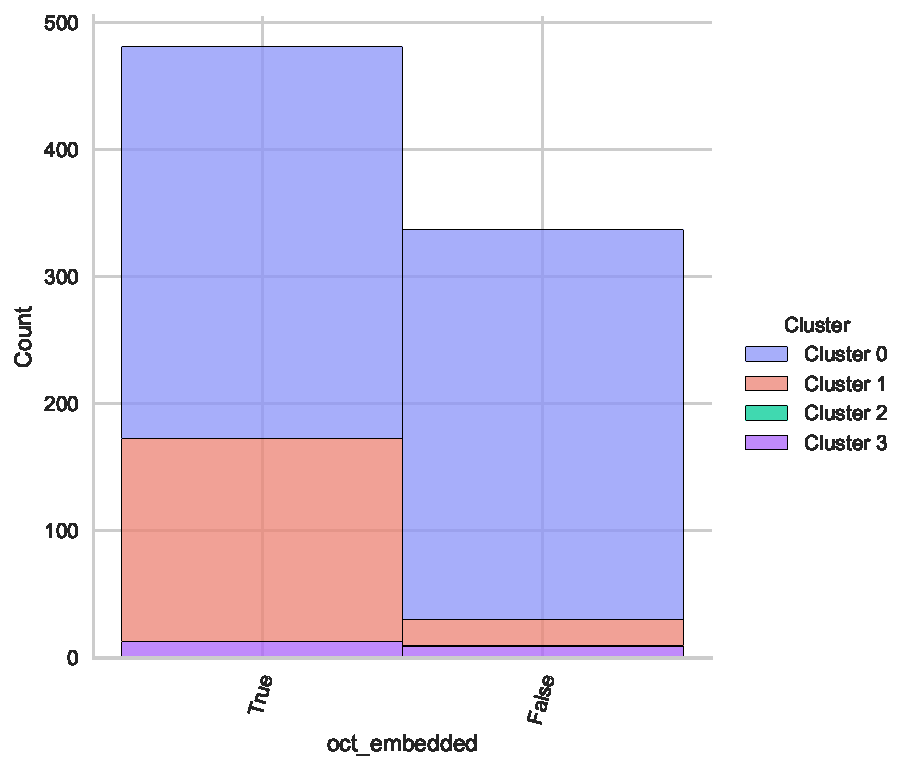
\includegraphics[width=0.22\textwidth]{NOTEBOOK/IMAGENES_BIRCH_DESCRIPTIVAS/28}
			\\  \hline 
			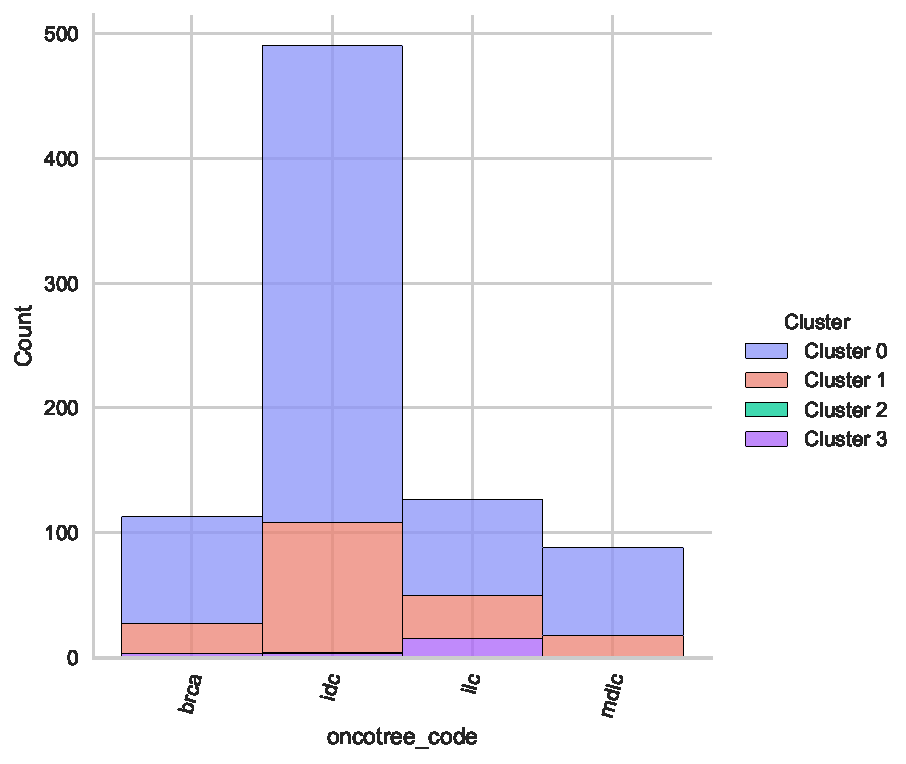
\includegraphics[width=0.22\textwidth]{NOTEBOOK/IMAGENES_BIRCH_DESCRIPTIVAS/29} 
			& 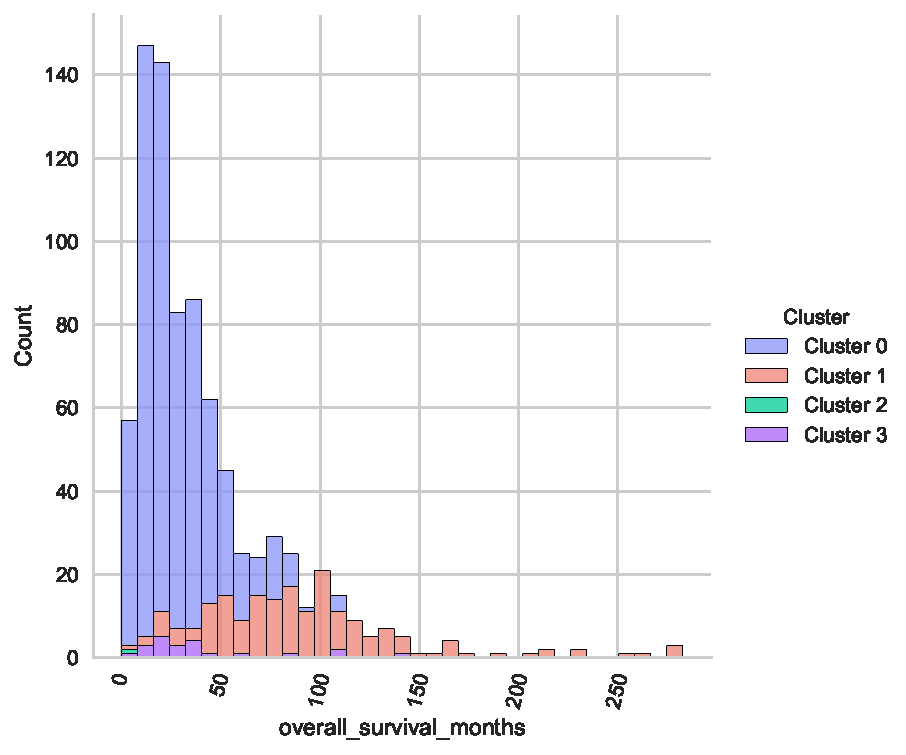
\includegraphics[width=0.22\textwidth]{NOTEBOOK/IMAGENES_BIRCH_DESCRIPTIVAS/30} 
			& 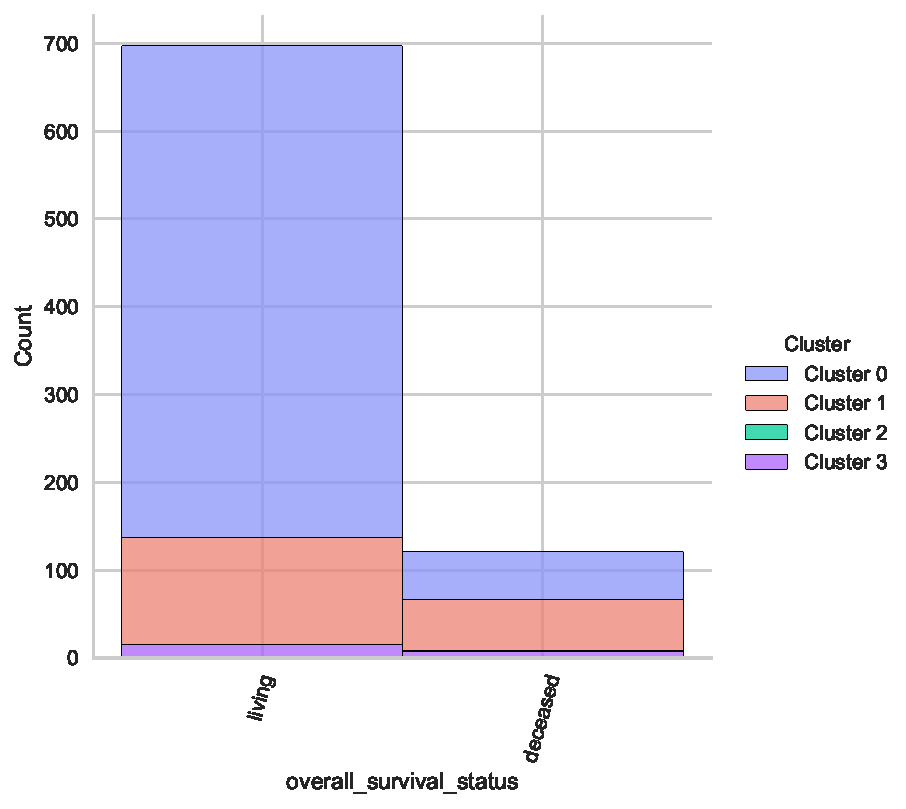
\includegraphics[width=0.22\textwidth]{NOTEBOOK/IMAGENES_BIRCH_DESCRIPTIVAS/31} 
			& 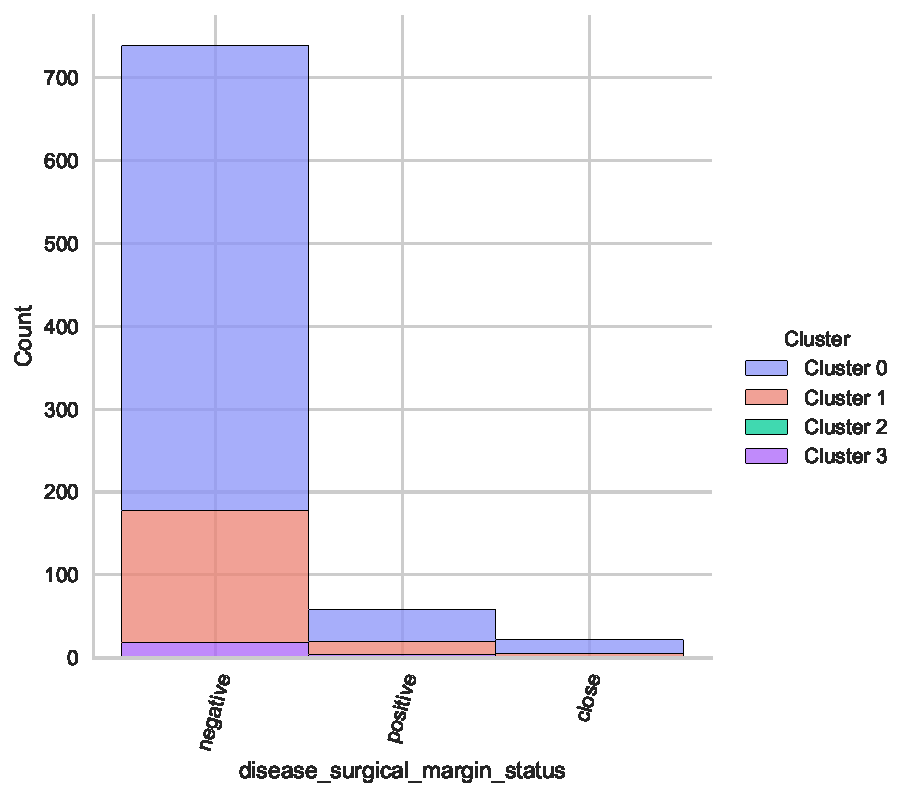
\includegraphics[width=0.22\textwidth]{NOTEBOOK/IMAGENES_BIRCH_DESCRIPTIVAS/32}
			\\  \hline 
			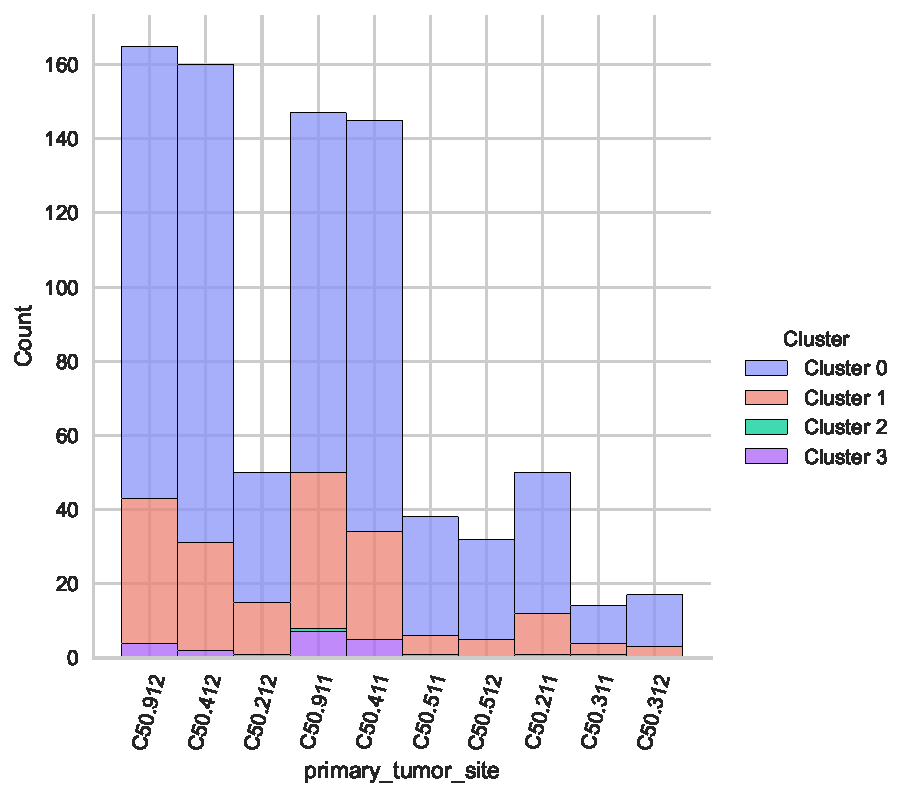
\includegraphics[width=0.22\textwidth]{NOTEBOOK/IMAGENES_BIRCH_DESCRIPTIVAS/33} 
			& 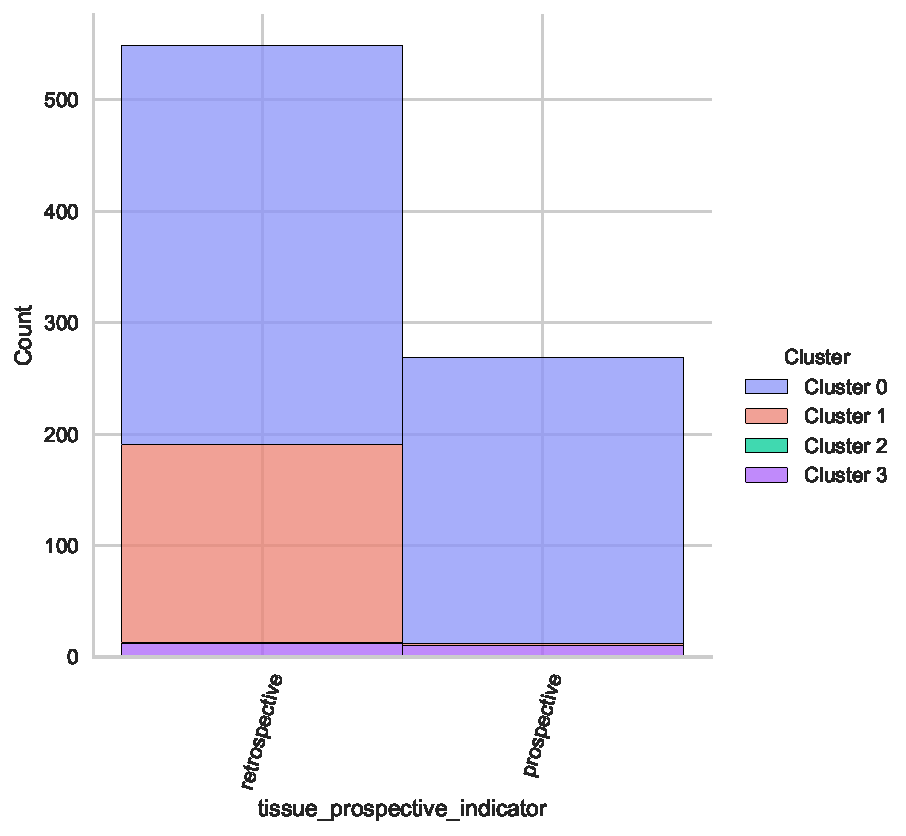
\includegraphics[width=0.22\textwidth]{NOTEBOOK/IMAGENES_BIRCH_DESCRIPTIVAS/34} 
			& 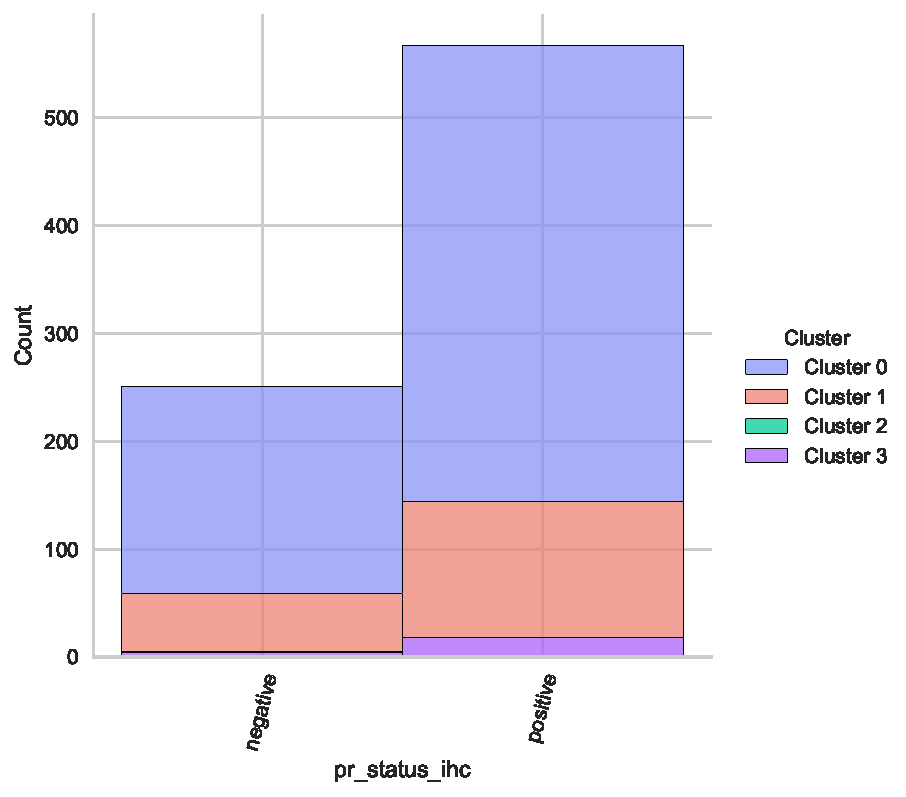
\includegraphics[width=0.22\textwidth]{NOTEBOOK/IMAGENES_BIRCH_DESCRIPTIVAS/35} 
			& 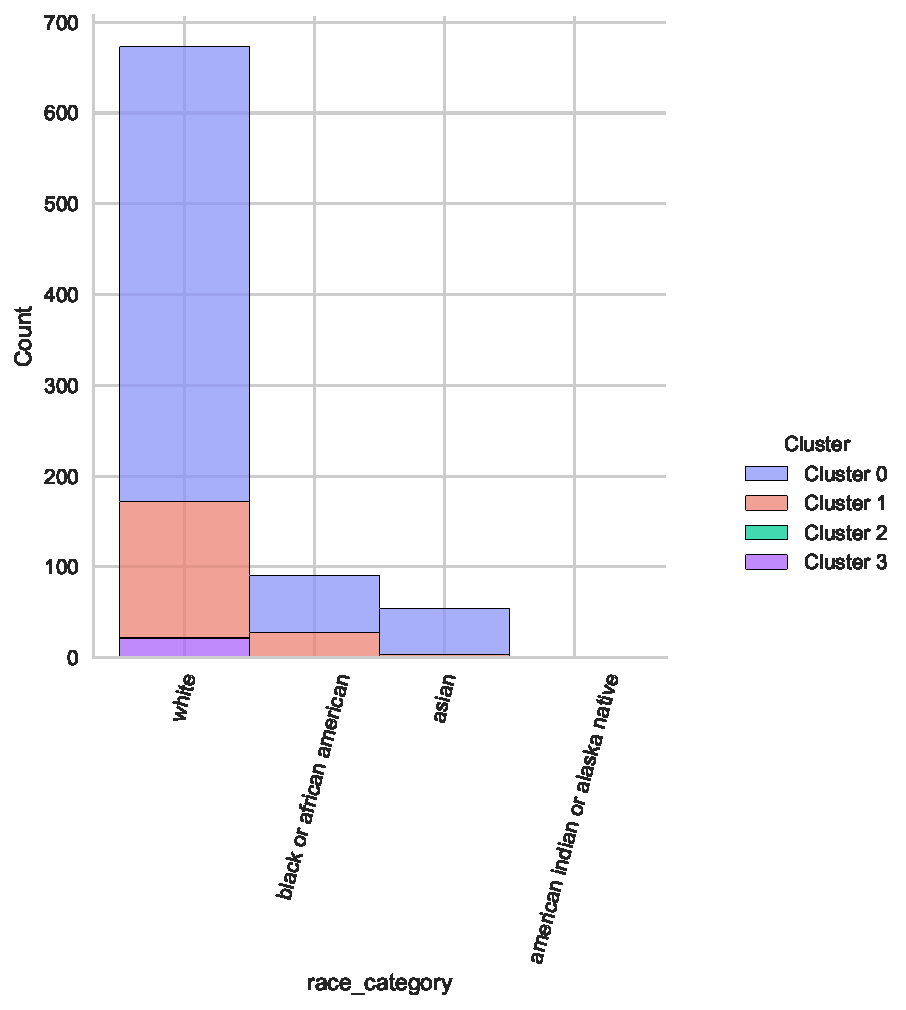
\includegraphics[width=0.22\textwidth]{NOTEBOOK/IMAGENES_BIRCH_DESCRIPTIVAS/36}         
			\\  \hline
			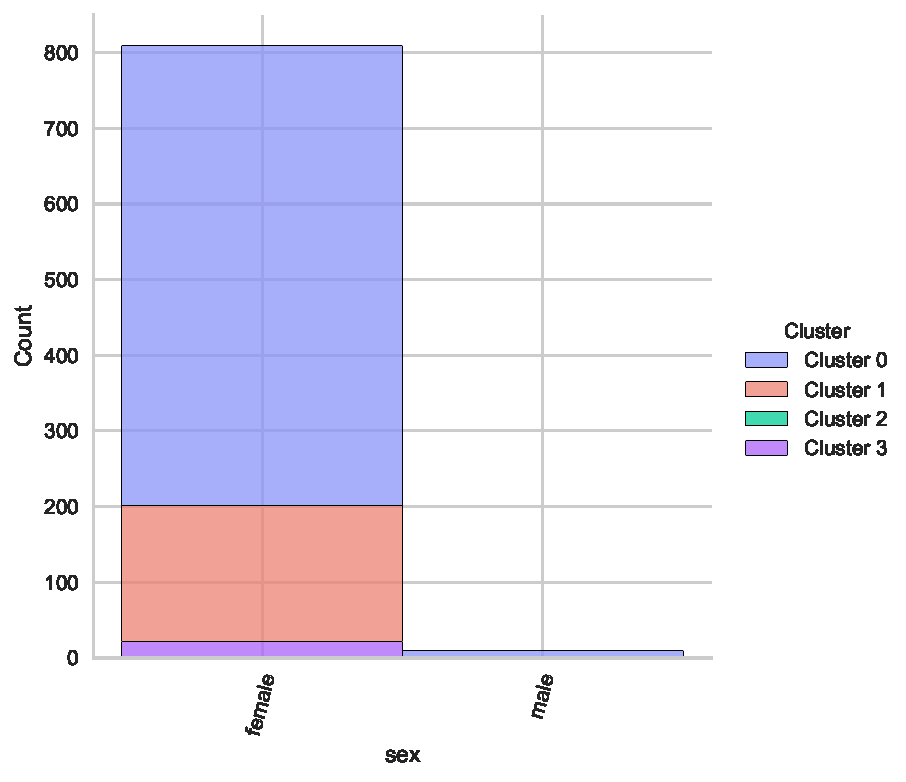
\includegraphics[width=0.22\textwidth]{NOTEBOOK/IMAGENES_BIRCH_DESCRIPTIVAS/37} 
			& 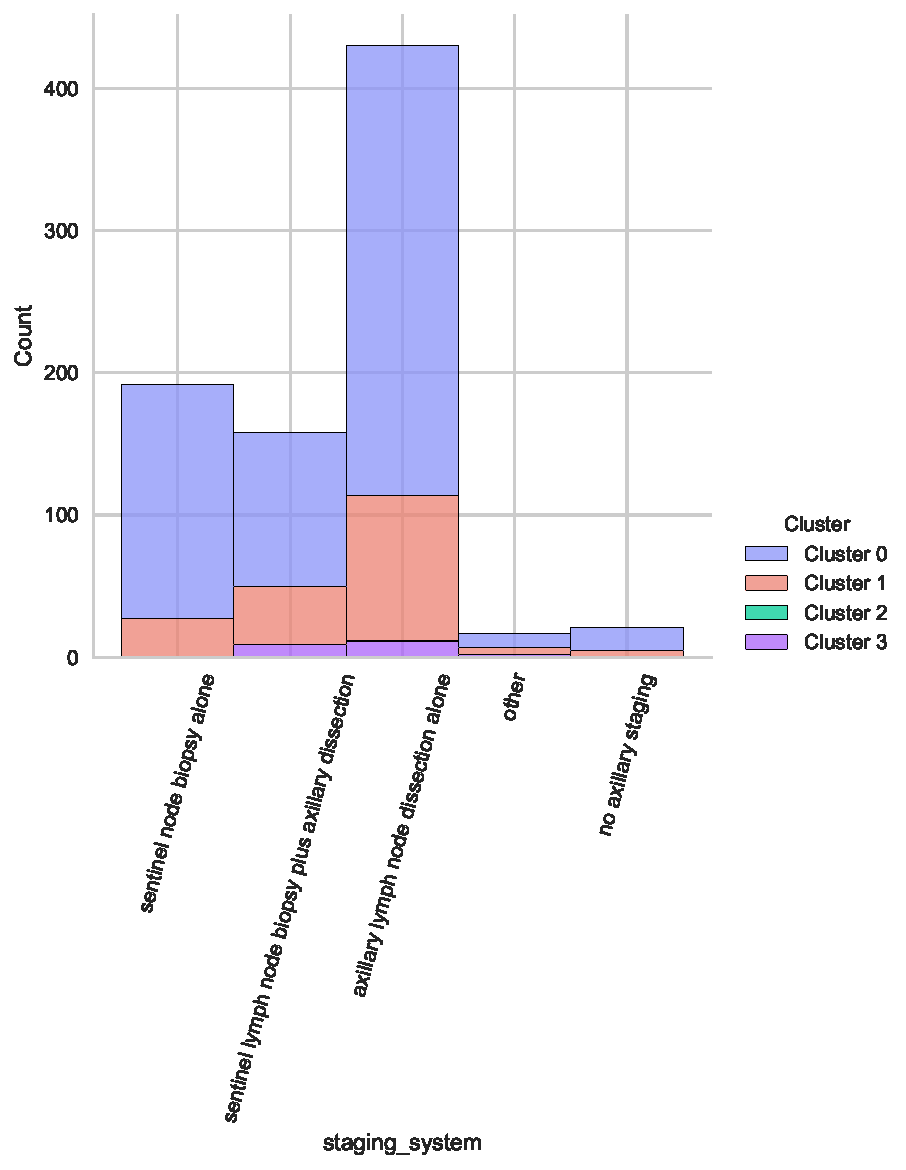
\includegraphics[width=0.22\textwidth]{NOTEBOOK/IMAGENES_BIRCH_DESCRIPTIVAS/38} 
			& 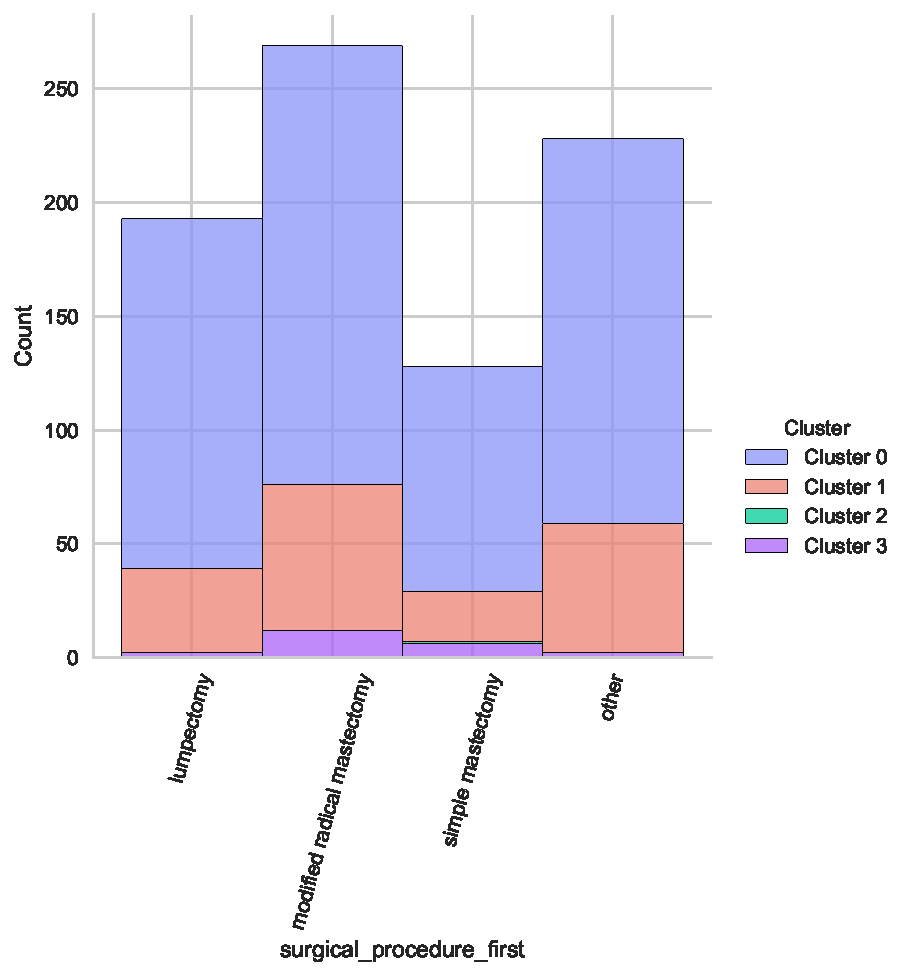
\includegraphics[width=0.22\textwidth]{NOTEBOOK/IMAGENES_BIRCH_DESCRIPTIVAS/39} 
			& 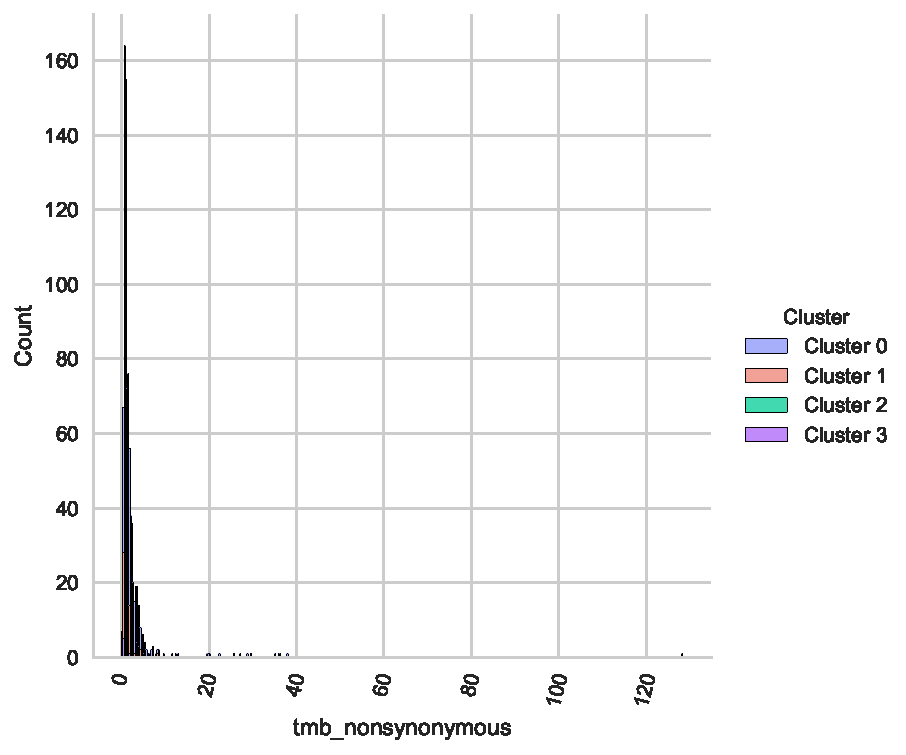
\includegraphics[width=0.22\textwidth]{NOTEBOOK/IMAGENES_BIRCH_DESCRIPTIVAS/40} 
			\\  \hline                  
		\end{tabular} 
		\caption{Clusters con características genómicas de 818 pacientes.}
		\label{clusters}
	\end{center} 
\end{table}
\break
Una vez analizados los resultados obtenidos, se observo que en los \textit {Cluster 0, 1 y 2} el Carcinoma Ductal Invasivo (IDC) era predominante en la mayoría de los pacientes, sin embargo, esta tendencia cambio en el \textit{Cluster 3} en donde el Carcinoma Lobulillar Invasivo (ILC) se presentó en la mayoría de los pacientes, tal y como se puede observar en la tabla \ref{carcinoma_cluster}. 
\begin{table}[!htb]
	\begin{center} 
		\begin{tabular}{ |c|c| }
			\hline 
			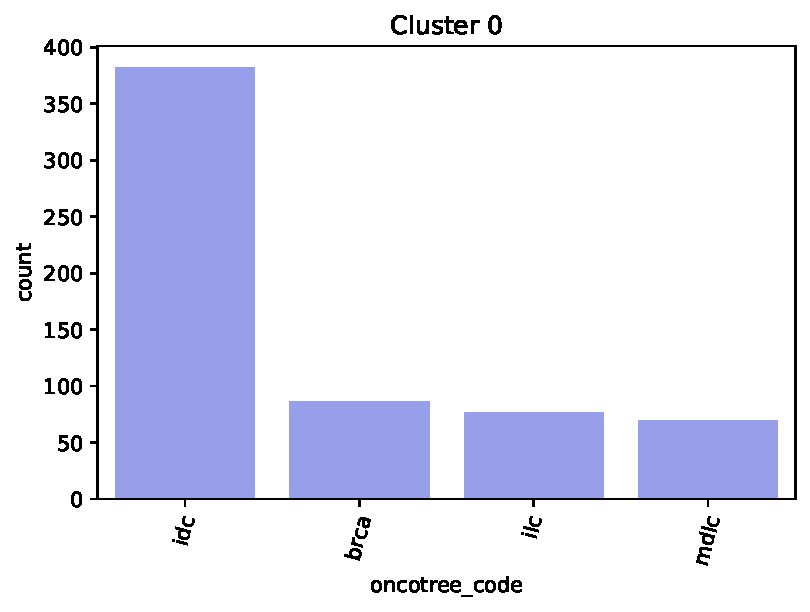
\includegraphics[width=.5\textwidth]{NOTEBOOK/IMAGENES_BIRCH_CLUSTERING/1_Cluster_0_oncotree_code} 
			& 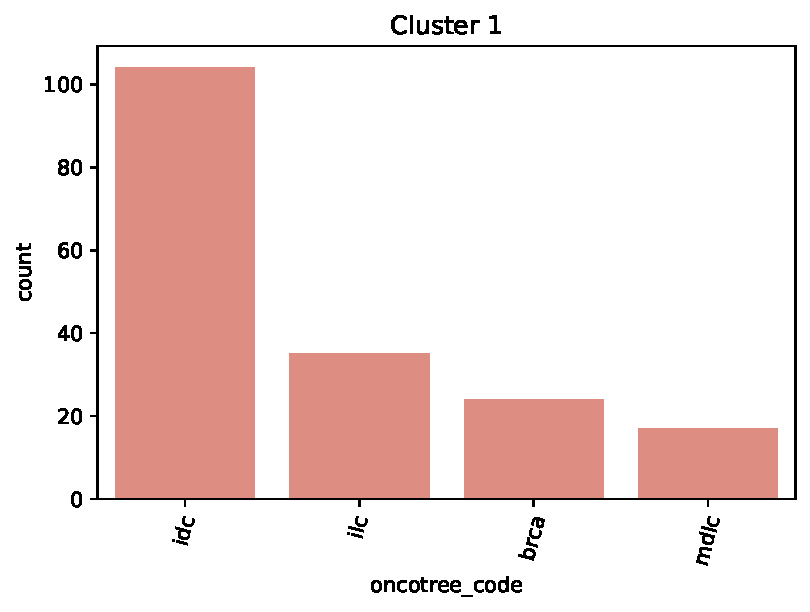
\includegraphics[width=.5\textwidth]{NOTEBOOK/IMAGENES_BIRCH_CLUSTERING/1_Cluster_1_oncotree_code} 
			\\  \hline
			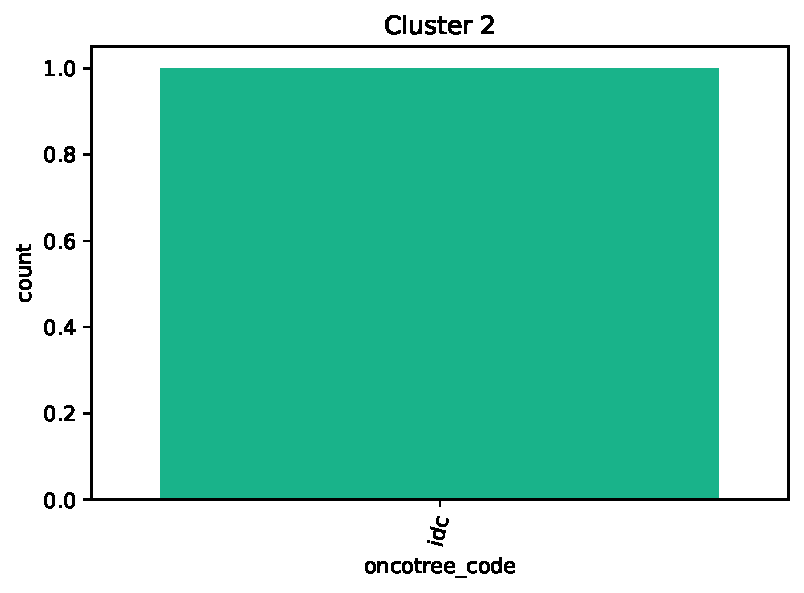
\includegraphics[width=.5\textwidth]{NOTEBOOK/IMAGENES_BIRCH_CLUSTERING/1_Cluster_2_oncotree_code} 
			& 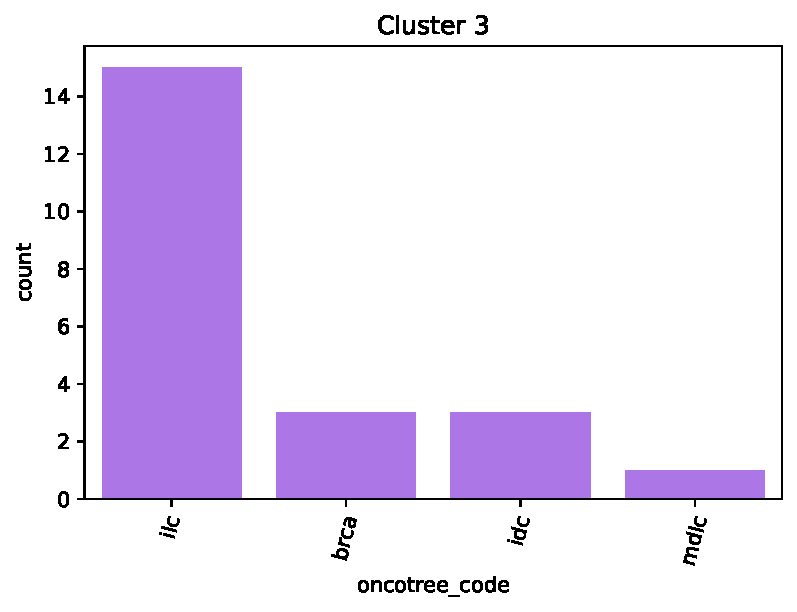
\includegraphics[width=.5\textwidth]{NOTEBOOK/IMAGENES_BIRCH_CLUSTERING/1_Cluster_3_oncotree_code} 
			\\  \hline            
		\end{tabular} 
		\caption{Clusters por tipo de carcinoma de mama.}
		\label{carcinoma_cluster}
	\end{center} 
\end{table}

Hay que mencionar que para poder determinar los atributos característicos se compararon las 41 variables de origen genómico de los 4 clusters. Se obtuvo como resultado, que 30 variables no presentaron cambio en ninguno de los clusters con respecto al análisis descriptivo realizado en las fases previas, sin embargo 9 variables presentaron diferencias en el \textit{Cluster 3} con respecto a los demás clusters, permitiéndonos identificar atributos genómicos inherentes del cáncer ILC con respecto al IDC. Llegados a este punto se infirió, según el comportamiento de los datos, las apreciaciones que se observan en la tabla \ref{interpretacion_BIRCH}:
\begin{table*}[htb!]
	\footnotesize
	\begin{threeparttable}
		\begin{tabular}{p{2.5cm} p{7cm} p{6.5cm}} \toprule
			\begin{center}Variable\end{center}   	 
			&\begin{center}Análisis descriptivo\end{center}             
			&\begin{center}Gráfico estadístico\end{center}\\ \hline
			%------------------------------------------------------	
			AJCC Neoplasm Disease Lymph Node Stage Code
			&  El código AJCC para la \textit{estadificación del cáncer por neoplasia del ganglio linfático(N)} presento el siguiente comportamiento en los clusters generados por el modelo BIRCH: La mayoría de los pacientes con IDC (Cluster 0) no manifestaron cáncer en los ganglios linfáticos cercanos, o el cáncer se diseminó de a 1 a 4 ganglios linfáticos debajo del brazo. Por el contrario, los pacientes con ILC (Cluster 3) presentaron metástasis tumoral en 10 o más ganglios linfáticos axilares. Por consiguiente, se infiere que el tipo de cáncer ILC presenta una mayor afectación y/o propagación hacia los ganglios linfáticos axilares cercanos al seno afectado en comparación con el cáncer IDC.
			
			& 
			\begin{center}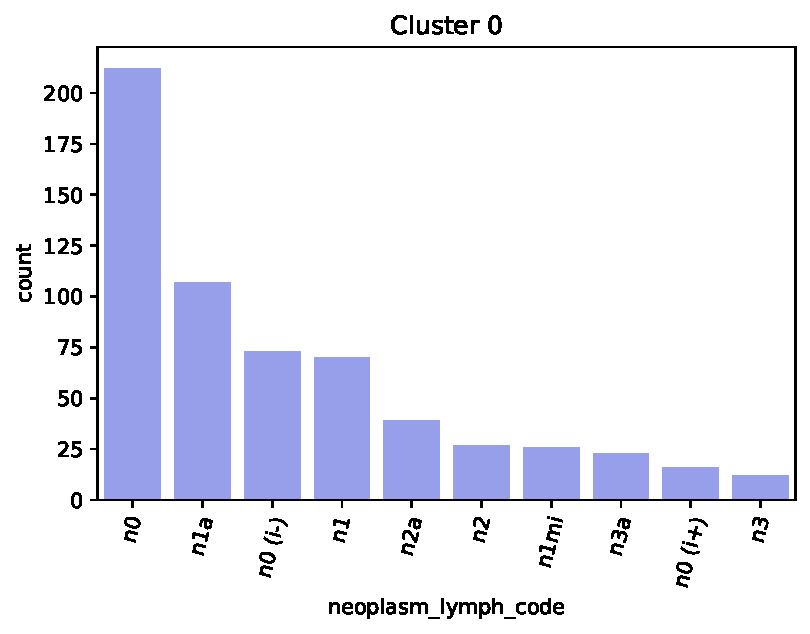
\includegraphics[width=1\linewidth]{NOTEBOOK/IMAGENES_BIRCH_CLUSTERING/2_Cluster_0_neoplasm_lymph_code}\end{center}
			\begin{center}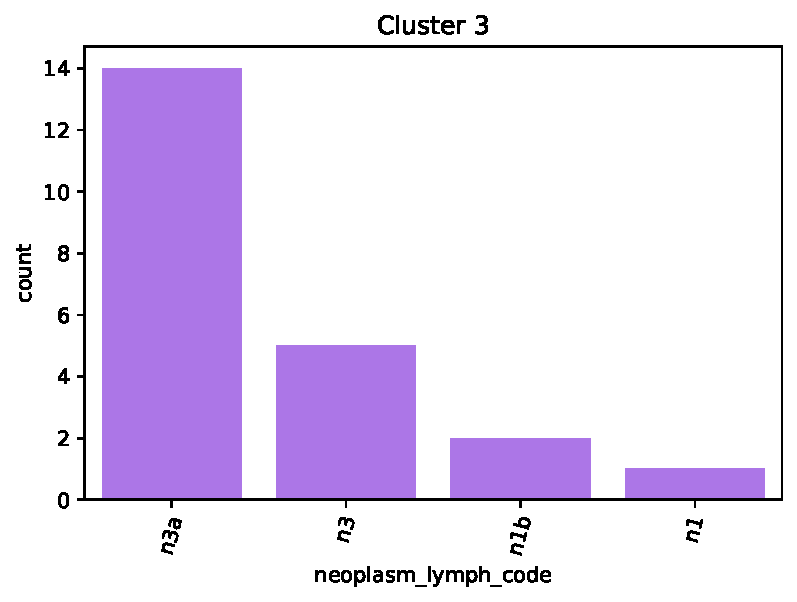
\includegraphics[width=1\linewidth]{NOTEBOOK/IMAGENES_BIRCH_CLUSTERING/2_Cluster_3_neoplasm_lymph_code}\end{center}
			
			\\ \hline
			%------------------------------------------------------	
			AJCC Neoplasm Disease Stage Code
			& Las etapas AJCC para la \textit{estadificación del cáncer por neoplasia} presentaron el siguiente comportamiento en los clusters generados por el modelo BIRCH: La mayoría de los pacientes con IDC (Cluster 0) el tumor mide 20 a 50 mm, y se propago de 1 a 3 ganglios linfáticos axilares. Por el contrario, en los pacientes con ILC (Cluster 3) el tumor es de cualquier tamaño y se diseminó a 10 o más ganglios linfáticos axilares, ganglios linfáticos mamarios internos y/o a los ganglios linfáticos debajo de la clavícula, sin embargo, no se propago a otras partes del cuerpo. Por consiguiente, se infiere que el tipo de cáncer ILC presenta un tamaño tumoral superior y una afectación considerable en ganglios linfáticos mamarios en comparación con el cáncer IDC.   
			
			& 
			\begin{center}\includegraphics[width=1\linewidth]{NOTEBOOK/IMAGENES_BIRCH_CLUSTERING/3_Cluster_0_neoplasm_disease_stage_code}\end{center}
			\begin{center}\includegraphics[width=1\linewidth]{NOTEBOOK/IMAGENES_BIRCH_CLUSTERING/3_Cluster_3_neoplasm_disease_stage_code}\end{center}
			
			\\ \hline
		\end{tabular}
	\end{threeparttable}
\end{table*}

\begin{table*}[htb!]
	\footnotesize
	\begin{threeparttable}
		\begin{tabular}{p{2.5cm} p{7cm} p{6.5cm}} \toprule
			%------------------------------------------------------	
			AJCC Tumor Stage Code 
			& 
			El código AJCC para la \textit{estadificación del tumor (T) primario del cáncer} presento el siguiente comportamiento en los clusters generados por el modelo BIRCH: En la mayoría de los pacientes con IDC (Cluster 0) el tumor tuvo un tamaño de 10 mm a 20 mm o menos. Por el contrario, en los pacientes con ILC (Cluster 3) se identificaron tumores que median más de 50 mm y además habían crecido dentro de la piel. Por consiguiente, se infiere que el tipo de cáncer ILC presenta un tamaño tumoral aproximadamente 2 veces más grande que del tipo de cáncer IDC. Cabe resaltar, que el cáncer IDC también presento pacientes con tumores mayores a 50 mm sin embargo su frecuencia de aparición no es tan alta como en el cáncer ILC en comparación con el cáncer IDC.
			& 
			\begin{center}\includegraphics[width=1\linewidth]{NOTEBOOK/IMAGENES_BIRCH_CLUSTERING/4_Cluster_0_tumor_stage_code}\end{center}
			\begin{center}\includegraphics[width=1\linewidth]{NOTEBOOK/IMAGENES_BIRCH_CLUSTERING/4_Cluster_3_tumor_stage_code}\end{center}
			
			\\ \hline
			%------------------------------------------------------	
			HER2 ihc percent positive
			& El \textit{Porcentaje positivo de HER2 según la prueba de inmunohistoquímica (IHC)}, presento el siguiente comportamiento en los clusters generados por el modelo BIRCH: En los pacientes con IDC (Cluster 0) el 91,06\% obtuvieron una tinción de membrana apenas perceptible, observada en un valor $<$\textit{10\%} de las células tumorales y el 8.94\% obtuvieron una tinción en un rango de moderada a intensa, observada en un valor de \textit{19-99\%} de las células tumorales. Por el contrario, en los pacientes con ILC (Cluster 3) el 95,45\%  obtuvieron una tinción de membrana apenas perceptible, observada en un valor $<$\textit{10\%} de las células tumorales y el 4.55\% de los pacientes obtuvieron una tinción intensa, observada en un valor de \textit{90-99\%} de las células tumorales. Por consiguiente, se infiere que en el tipo de cáncer ILC el porcentaje positivo de HER2 es más difícil de identificar debido a que la mayoría de células tumorales presentan una tinción de membrana apenas perceptible en comparación con el cáncer IDC.
			
			& 
			\begin{center}\includegraphics[width=1\linewidth]{NOTEBOOK/IMAGENES_BIRCH_CLUSTERING/5_Cluster_0_her_2_ihc_percent_positive}\end{center}
			\begin{center}\includegraphics[width=1\linewidth]{NOTEBOOK/IMAGENES_BIRCH_CLUSTERING/5_Cluster_3_her_2_ihc_percent_positive}\end{center}
			
			\\ \hline
		\end{tabular}
	\end{threeparttable}
\end{table*}
\begin{table*}[htb!]
	\footnotesize
	\begin{threeparttable}
		\begin{tabular}{p{2.5cm} p{7cm} p{6.5cm}} \toprule
			%------------------------------------------------------	
			Primary Lymph Node Presentation Assessment Ind-3
			& La \textit{Evaluación de los ganglios linfáticos} presento el siguiente comportamiento en los clusters generados por el modelo BIRCH: En los pacientes con IDC (Cluster 0), el 97,25\% se diagnosticó con afectación metastásica en los ganglios linfáticos axilares y el 2.76\% no manifestó señales de enfermedad metastásica. Por el contrario, en los pacientes con ILC (Cluster 3) todos se diagnosticaron con afectación metastásica en los ganglios linfáticos axilares. Por consiguiente, se infiere el tipo de cáncer ILC genera una mayor afectación metastásica en los ganglios linfáticos mamarios. Cabe resaltar, que el cáncer IDC también genero una afectación metastásica considerable en los ganglios linfáticos, sin embargo, en una parte de los pacientes no genero un comportamiento metastásico constante, por lo que es posible inferir que a diferencia del ILC su propagación es menor en los ganglios linfáticos mamarios. 
			& 
			\begin{center}\includegraphics[width=1\linewidth]{NOTEBOOK/IMAGENES_BIRCH_CLUSTERING/6_Cluster_0_lymph_presentation}\end{center}
			\begin{center}\includegraphics[width=1\linewidth]{NOTEBOOK/IMAGENES_BIRCH_CLUSTERING/6_Cluster_3_lymph_presentation}\end{center}
			
			\\ \hline
			%------------------------------------------------------	
			Positive Finding Lymph Node Hematoxylin and Eosin Staining Microscopy Count
			& El \textit{recuento de ganglios linfáticos positivos identificados mediante microscopía óptica con tinción de hematoxilina y eosina (H\&E)} presento el siguiente comportamiento en los clusters generados por el modelo BIRCH: En los pacientes con IDC (Cluster 0), se generó una tendencia central aproximada de 5 ganglios linfáticos con H\&E positivo, es decir que la tinción de hematoxilina presento una mayor proporción evidenciando la presencia de un tumor en crecimiento. Adicionalmente, se pudo observar que el valor mínimo ganglios linfáticos afectados fue 1 y el valor máximo de ganglios linfáticos afectados fue 19. Por el contrario, en los pacientes con ILC (Cluster 3), se generó una tendencia central aproximada de 23 ganglios linfáticos con H\&E positivo. Adicionalmente, se pudo observar que el valor mínimo ganglios linfáticos afectados fue 12 y el valor máximo de ganglios linfáticos afectados fue 35. Por consiguiente, se infiere que el tipo de cáncer ILC afecta de manera significativa una mayor cantidad ganglios linfáticos e incentiva el crecimiento de los tumores en comparación con el tipo de cáncer IDC.
			
			& 
			\begin{center}\includegraphics[width=1\linewidth]{NOTEBOOK/IMAGENES_BIRCH_CLUSTERING/7_Cluster_0_positive_lymph_hematoxylin}\end{center}
			\begin{center}\includegraphics[width=1\linewidth]{NOTEBOOK/IMAGENES_BIRCH_CLUSTERING/7_Cluster_3_positive_lymph_hematoxylin}\end{center}
			
			\\ \hline
		\end{tabular}
	\end{threeparttable}
\end{table*}

\begin{table*}
	\footnotesize
	\begin{threeparttable}
		\begin{tabular}{p{2.5cm} p{7cm} p{6.5cm}} \toprule
			%------------------------------------------------------	
			Mutation Count
			&  El \textit{recuento de mutaciones} en el ADN, el cual ocasiona que una célula sana crezca y se divida con mayor rapidez, presento el siguiente comportamiento en los clusters generados por el modelo BIRCH:  En los pacientes con IDC (Cluster 0), se generó una tendencia central aproximada de 38 mutaciones, en donde el número mínimo de mutaciones es 1 y el número máximo de mutaciones es 1135. Por el contrario, en los pacientes con ILC (Cluster 3), se generó una tendencia central aproximada de 28 mutaciones, en donde el número mínimo de mutaciones es 12 y el número máximo de mutaciones es 84. Por consiguiente, se infiere que el tipo de cáncer ILC presenta un menor grado de crecimiento de las células sanas y se divide de una forma tardía en comparación con el cáncer IDC. Por lo tanto, es plausible afirmar, que el aumento anormal del tejido graso y fibroso en el seno es suficiente para el tipo cáncer IDC pero no necesario para el tipo de cáncer ILC. 
			& 
			\begin{center}\includegraphics[width=1\linewidth]{NOTEBOOK/IMAGENES_BIRCH_CLUSTERING/8_Cluster_0_mutation_count}\end{center}
			\begin{center}\includegraphics[width=1\linewidth]{NOTEBOOK/IMAGENES_BIRCH_CLUSTERING/8_Cluster_3_mutation_count}\end{center}
			
			\\ \hline
			%------------------------------------------------------	
			Overall Survival (Months)
			& La \textit{Supervivencia general} presento el siguiente comportamiento en los clusters generados por el modelo BIRCH: En los pacientes con IDC (Cluster 0), se tiene una tendencia central aproximada de 23 meses (2 años), en donde el tiempo mínimo de supervivencia es 5 meses y el tiempo máximo de supervivencia es 112 meses (10 años). Por el contrario, en los pacientes con ILC (Cluster 3), se tiene una tendencia central aproximada de 28 meses (2 años y medio), en donde el tiempo mínimo de supervivencia es 7 meses y el tiempo máximo de supervivencia es 139 meses (12 años). Por consiguiente, se infiere que el tipo de cáncer ILC se propaga de manera más lenta en comparación con el tipo cáncer IDC. Por lo tanto es plausible afirmar, que el diagnóstico del cáncer IDC afecta de forma significativa la detección del cáncer ILC debido a que presenta una propagación más rápida, una tasa de supervivencia menor en los pacientes y un crecimiento acelerado del tejido mamario que dificulta la localización y visibilidad del cáncer ILC. 
			
			& 
			\begin{center}\includegraphics[width=1\linewidth]{NOTEBOOK/IMAGENES_BIRCH_CLUSTERING/9_Cluster_0_overall_survival_months}\end{center}
			\begin{center}\includegraphics[width=1\linewidth]{NOTEBOOK/IMAGENES_BIRCH_CLUSTERING/9_Cluster_3_overall_survival_months}\end{center}
			
			\\ \hline
		\end{tabular}
	\end{threeparttable}
\end{table*}
\clearpage
\begin{table*}
	\footnotesize
	\begin{threeparttable}
		\begin{tabular}{p{2.5cm} p{7cm} p{6.5cm}} \toprule
			%------------------------------------------------------	
			TMB
			& La \textit{Carga mutacional tumoral (TMB)} presento el siguiente comportamiento en los clusters generados por el modelo BIRCH: En los pacientes con IDC (Cluster 0), se tiene una tendencia central de $1.3$ $mut/mb$ en donde el valor mínimo es $0.5$ $mut/mb$ y el valor máximo $37.9$ $mut/mb$. Por el contrario, en los pacientes con ILC (Cluster 3), se tiene una tendencia central de $0.9$ $mut/mb$ en donde el valor mínimo es $0.4$ $mut/mb$ y el valor máximo $3.2$ $mut/mb$. Por consiguiente, se infiere que los pacientes con ILC tienen un valor bajo de TMB, es decir, que generan una menor cantidad de neoantígenos, lo que hace que los tumores sean menos inmunogénicos a los tratamientos en comparación con el tipo de cáncer IDC. De manera que para los pacientes con cáncer ILC existe una probabilidad más alta de curarse de cáncer de mama en comparación con el cáncer IDC.  
			
			& 
			\begin{center}\includegraphics[width=1\linewidth]{NOTEBOOK/IMAGENES_BIRCH_CLUSTERING/10_Cluster_0_tmb_nonsynonymous}\end{center}
			\begin{center}\includegraphics[width=1\linewidth]{NOTEBOOK/IMAGENES_BIRCH_CLUSTERING/10_Cluster_3_tmb_nonsynonymous}\end{center}
			
			\\ \hline
		\end{tabular}
		\caption{Interpretación de los clusters obtenidos con el modelo BIRCH a partir del conjunto de datos del Carcinoma invasivo de mama (TCGA, Cell 2015).}
		\label{interpretacion_BIRCH}
	\end{threeparttable}
\end{table*}
\clearpage
